  
\RequirePackage[l2tabu, orthodox]{nag}

\documentclass[review, glossary]{thesis}

\def\UrlBreaks{\do\/\do-}

\usepackage{array}
\newcolumntype{P}[1]{>{\centering\arraybackslash}p{#1}}

\usepackage{amsmath, amsfonts, amsthm, amssymb, commath}
\usepackage{boxedminipage, xspace}   
\usepackage[T1]{fontenc}
\usepackage{changepage}
\usepackage[export]{adjustbox}

\usepackage{graphics, graphicx}
\usepackage{subfig}

\usepackage{booktabs}
\usepackage{multirow}
\usepackage{parcolumns}
\usepackage[roman]{parnotes}

\usepackage{algorithm}
\usepackage{algorithmic}

\usepackage{color}
\usepackage{listings}
\usepackage{framed}

\definecolor{keyword}{RGB}{127,0,0}
\definecolor{block}{RGB}{0,127,0}
\definecolor{variable}{RGB}{0,0,127}

\lstset{
numbers=left,
stepnumber=1,
numbersep=5pt,
xleftmargin=0pt,
xrightmargin=0pt,
breaklines=true,
escapeinside={<@}{@>},
numberstyle=\color{black},
columns=fixed,
keepspaces=true,
columns=flexible,
framesep=0pt,
frame=single,
basicstyle=\ttfamily\footnotesize
}


\addbibresource{references.bib}

\begin{document}		
	\frontmatter
	\pagenumbering{gobble}
	
	\thispagestyle{empty}
\newgeometry{left=2cm,right=2cm,top=2cm,bottom=0.1cm}

\begin{center}         
         
\includegraphics[width=0.2\linewidth]{figures/logo/logoul.pdf}
         \vspace{0.3cm}\noindent
%         \texttt{PhD-FSTC-2016-43}
         
         The Faculty of Science, Technology and Communication
         
         \vspace{1cm}\noindent
         {\LARGE \textbf{\textsc{Dissertation}}}
         
         \vspace{0.5cm}
         \noindent
         Defense held on September $15^{th}$, 2021 in Luxembourg
         
         \vspace{0.5cm}\noindent
         to obtain the degree of
         
         \vspace{0.8cm}\noindent
         {\large \textbf{\textsc{Docteur de l'Université du Luxembourg en Informatique}}}

         \vspace{0.5cm}\noindent
         {\Large by}

         \vspace{0.5cm}\noindent
         {\Large Renaud \textsc{Rwemalika}}\\
%         {\footnotesize Born on $24^{th}$ November 1992 in Libourne (France)}

         \vspace{1cm}\noindent
         {\LARGE \textbf{\textsc{On the Maintenance of}}}\\[0.4cm] 
         {\LARGE \textbf{\textsc{System User Interactive Tests}}}\\[0.4cm]
\end{center}

\vspace{0.4cm}

\begin{adjustwidth*}{1em}{1em}

\noindent
\textbf{\large Dissertation defence committee}
%\normalsize\textit{(Waiting for approval)}


\vspace{0.2cm}
\noindent
Dr.  Marinos \textsc{Kintis}, advisor\\
{\small \emph{Senior Data Engineer, FanDuel, United Kingdom}}   

\vspace{0.2cm}
\noindent
Dr. Michail \textsc{Papadakis}, advisor\\
{\small \emph{Lecturer, University of Luxembourg, Luxembourg, Luxembourg}}   

\vspace{0.2cm}
\noindent
Prof. Dr. Yves \textsc{Le Traon}, supervisor\\
{\small \emph{Professor, University of Luxembourg, Luxembourg, Luxembourg}}

\vspace{0.2cm}
\noindent
Prof. Dr. Myra \textsc{Cohen}, supervisor\\
{\small \emph{Professor, Iowa State University, Ames, Iowa}}

\vspace{0.2cm}
\noindent
Prof. Dr. Anna Rita \textsc{Fasolino}, supervisor\\
{\small \emph{Professor, Iowa State University, Luxembourg, Luxembourg}}

\end{adjustwidth*}

\restoregeometry
	
	\linenumbers
	\chapter*{Abstract}

Many companies rely on software testing to verify that their software products meet their requirements. However, test quality and, in particular, the quality of tests interacting with the \gls{gui}, i.e. \gls{suit}, is hard to achieve. The problem becomes challenging when the \gls{sut} evolves, as \gls{suit} suites need to adapt and conform to the evolved software. Indeed, because the user interface is a part of the system that tends to undergo rapid evolutions, \gls{suit}s are particularly prompt to break.

In this dissertation, we present an empirical evaluation of the impact of the evolution and the maintenance of SUIT suites. We aim to demonstrate the problem of test maintenance and overall improve the understanding of SUIT scripts evolution. To that end, we identify, collect and analyze test code changes across the evolution of an industrial test suite. We show that the problem of test maintenance is largely due to test fragility (most commonly performed changes are due to locator and synchronization issues) and bad practices (over 30\% of keywords are duplicated). 

To further investigate the question of bad test code practices such as test clones, we perform a multivocal study to identify which bad practices, i.e. SUIT smells, are already studied in both industry and academia establish a list of 35 test code smells. For 16 of them, we derive metrics to analyze their diffusion across tests as well as potential refactoring actions removing the test code smells. Conducting a second empirical study, including both industrial and open-source test suites, we show that test code smells are largely present in \gls{suit}s, potentially contributing to the fragility and hindering the maintenance process. Interestingly, when observing refactoring actions, they remain rare during the lifespan of the tests. Yet, symptoms tend to disappear as old tests are discarded and new ones are introduced.

However, during the analysis of SUIT smells, we observe that bad practices impacting locators do not appear often in the test code. This observation contrasts with the analysis of the evolution of the SUIT presented in our first empirical study.  This apparent contradiction arises from the limitation of property-based locators which rely on the structure of the representation layer of the \gls{sut}. Thus, such approaches are sensitive to internal iso-functional changes occurring during the normal evolution of the \gls{sut}. To account for this limitation, we introduce a new way of expressing locators, HPath. Instead of relying on the internal representation of the GUI, HPath relies on its rendered characteristics. Our results suggest that despite what is presented in the literature on smells, locators relying on a smaller number of GUI elements to fully qualify a target do not necessarily lead to more robust locators. On the contrary, the choice of the GUI element properties seems to play a stronger role in the robustness to change.

Overall, this dissertation provides insights into how \gls{suit}s evolve and shows that \gls{suit} fragility plays a major role in the associated maintenance effort. It also proposes techniques that effectively facilitate the maintenance with the early detection of sub-optimal patterns and the introduction of a locator representation more robust to \gls{sut} evolution.
	
	\tableofcontents
	
	\cleardoublepage
	
	\mainmatter	
	
	\chapter{Introduction}
\label{chap:introduction}

\chapterPage{
With GUI-based applications becoming ubiquitous as a mean for users to interact with software, the question of their correctness is of utmost importance. Yet, testing such applications still poses major challenges to practitioners. 
After introducing four approaches employed when creating \gls{suit}, we introduce the challenges that come with them.
Before describing the three contributions of this dissertation, we scope the addressed sub-challenges tackled.
}

Today, companies need to produce software faster than ever in order to remain competitive. To do so, they rely mainly on two different strategies: the integration of a continuous deployment pipeline and the establishment of agile methodologies within the company. These strategies allow software producers to increase the release rate while maintaining a high quality for the software that is shipped.

One of the keystones of the quality process is based on the adoption of strategies to assess that both functional and technical requirements are met. Because of the complex dynamic runtime of most modern applications, static analysis techniques face limitations in revealing violations of the requirements. Thus, most teams heavily rely on testing to reveal faults in their software. 

We define testing as a technical investigation to assess the quality of a \gls{sut} by executing the latter against a set of input values. Tests can further be classified through the scope they target into three main categories: unit, integration, and system tests. Unit testing covers the tests that are testing a unit in isolation, be it a class, a function, or any other software component,  to validate each unit individually. In integration testing, related units are grouped together and tested as a group. Finally, system testing covers the tests evaluating the system as a whole to ensure its compliance with its requirements.

Because unit and integration tests target more restricted portions of the application, they offer better control to the tester who can isolate functionalities from its environment and tests specific behaviors of the system sub-parts. On the other hand, system tests, and especially those interacting with the user interface, target the system as a whole (usually as a black box). Therefore, they are sensitive to any change in the \gls{sut} and its interface. This property makes system tests more fragile, \ie\ they may break as a result of non-functional changes that are not targeted by the test.

In this work, we analyze the evolution of those system tests interacting with the user interface to shed light on the reasons why these tests require costly maintenance \cite{Alegroth2016, Coppola2020}. Then, we propose some solutions as to how to create more robust test suites, \ie test suites that are less likely to break following non-functional evolutions of the \gls{sut}.

\section{GUI Testing}
\label{sec:introduction-gui-testing}

User Interfaces are designed to provide a mean for the user to interact with an application. Unfortunately, as interfaces become more user-friendly, the underlying technology becomes more complex \cite{Myers1994}. Indeed, as depicted by \textcite{Myers1995}, user interfaces require the system to  interact with complex graphical components, to provide multiple ways to provide the same command, to manage multiple asynchronous input devices through the use of asynchronous event loops, or to provide an interactive computer programming environment (\eg\ read–evaluate–print loop). To ease development, the literature introduces different architectural designs to decouple the code responsible for the user interaction from the rest of the system such as the Entity-Component-System model \cite{Raffaillac2018} or the Model-View-Controller \cite{Krasner1988}.

Nevertheless, while these architectural solutions offer advantages by providing better isolation when testing individual components, in the case of system testing, the challenges remain open. Indeed, as the complexity of user interfaces and their associated code continues to grow, testing through the user interface for functional correctness remains challenging, but vital to help ensure the safety, robustness, and usability of the \gls{sut}.

Furthermore, today, \gls{gui} are becoming ubiquitous as a mean for users to interact with a software application \cite{Myers1992, Myers1995, Brooks2009, Memon2010}. In this work, we define a \gls{gui} as a hierarchical, graphical front-end to a software system that accepts as input user-generated and system-generated events from a fixed set of events that result in graphical output \cite{Memon2007} and/or alter the state of the software \cite{Nguyen2014}. A \gls{gui}-based application is a software for which the \gls{gui} is the main mode of interaction to the detriment of other types of user interfaces. As a consequence of the predominance of \gls{gui}-based applications, a lot of effort has been geared towards \gls{gui} automation, notably focusing on desktop applications \cite{Nguyen2014, Advolodkin2018, Pezze2018}, web applications \cite{Mesbah2009, Biagiola2019}, mobile applications \cite{Machiry2013, Gomez2013, Mao2016, Salihu2019, Yu2019} or cross-platform applications \cite{Canny2020}. However, as we show later in this section, major challenges remain open.

The question of the correctness of a \gls{gui}-based application is of utmost importance since prototyping and developing the behavior of a system is harder than prototyping and developing the appearance of the application \cite{Myers2008}. It is in this context that we introduce \gls{gui} testing which encompasses the techniques used to test user interface layout and its behavior. More precisely, \gls{gui} testing can be defined as ``the process of testing a software application with a graphical front-end to guarantee that it meets its specification by performing a sequence of events against the \gls{gui} elements'' \cite{Cunha2010, Banerjee2013, Issa2012}. Thus, relying only on stimuli inputs and output reactions, a \gls{gui} test is considered as a black-box test. Additionally, we define a \gls{suit} as an automated \gls{gui} test that exercises the \gls{sut} as a whole (system level). Note that in this work focusing on automated system-level test interacting with the \gls{sut} through its \gls{gui}, we use \gls{gui} test and \gls{suit} interchangeably.

Strategies have been developed to exercise the user interface to ensure that functional requirements are satisfied. Different techniques have been proposed but all rely on the same principle. A test framework executes events belonging to \gls{gui} components and monitors the resulting changes to the program state \cite{Nguyen2014}. In other words, each technique generates a sequence of test step, that will be executed against the \gls{sut} (input) and captures some indication as to what is the current state of the system (output). Each test step consists of a triple: (1) an action to be performed, (2) the \gls{gui} element on which to perform the action, and (3) an optional value passed to the element. Consequently, a natural classification discriminates each strategy on the way the sequence of test steps is generated.

In the remainder of this section, we discuss current techniques used to generate \gls{suit}s. The techniques are ordered based on their theoretical potential for automation during the test generation process.

\subsection{Random GUI Testing}
\label{sec:introduction-random-gui-testing}

In random \gls{gui} testing, also known as monkey testing or random-walk, tests are automatically created by generating sequences of events at random in the hope of exploring the \gls{sut} to reveal failures. Because no requirements are passed as input such techniques rely on specific constraints that are application or domain invariant oracles \cite{Mesbah2009} to assess correctness. Thus, any sequence of events that causes the \gls{sut} to violate an invariant is considered as a fault revealing test case \cite{Barr2015}. These properties make random \gls{gui} testing cheap to run on a large number of versions/configurations of applications.

Typically, such tools rely on the concept of fuzz testing which performs arbitrary or contextual events against the SUT. Tools like Monkey \cite{Google2020},  ATUSA \cite{Mesbah2012} or Dynodroid \cite{Machiry2013} rely on pseudo-random input events which include both user interface events and system events and assess the generated sequences against invariant oracles. 

One of the major challenges encountered when relying on random \gls{gui} testing resides in the exploration of the application states. Indeed, with modern applications, the infinite number of combinations of user inputs leads to a potentially large and sometimes infinite number of reachable states. Consequently, the search space cannot be covered exhaustively leading to potentially low state coverage \cite{Canny2019}. Furthermore, in the case of more complex input, such as a chain of character, randomly generated input have often low chances of producing feasible test cases, thus requiring a large number of input generations to find interesting test cases (\eg if a login page exists, only a combination of a valid user name and password would allow the test case to continue its exploration behind the login wall).

To alleviate these limitations, different approaches emerged introducing algorithms relying on heuristics to better explore the application state space and consequently generate more fault-revealing test cases. For example, EXSYST \cite{Gross2012}, EvoDroid \cite{Mahmood2014} and Sapienz \cite{Mao2016} propose to use search-based algorithms to explore the space of possible sequences and generate tests for Android applications while Dynodroid \cite{Machiry2013} exploits machine learning algorithms to achieve the same goal. The goal of the algorithm is to generate short sequences of input while improving coverage (code \cite{Gross2012} and/or state \cite{Machiry2013} coverage) to produce fault-revealing sequences. More recently, tools such as DIG \cite{Biagiola2019} try to increase the coverage by specifically targeting the input generation problem. While these approaches look promising, today, monkey testing requires the user to provide some inputs (\eg login and passwords) to allow the algorithms to explore more states.

To summarize, random \gls{gui} testing offers a cheap alternative to classical test scripting which can be useful to detect crashes and other invariants in an exploratory fashion. Nevertheless, because of the lack of knowledge of the functional requirements and the lifecycle of the application, exploring the application and covering hidden behaviors remains challenging. Thus, while companies do use random \gls{gui} testing, they use it in addition to other techniques that we present below.

\subsection{Model-Based Testing}
\label{sec:introduction-model-based-testing}

\gls{mbt} is an approach encompassing the processes and techniques for the automatic derivation of abstract test cases from abstract models \cite{Utting2012}. Functional specifications of a system, with the assumption that they are precise enough, are used as input to design process models which in turn are used to generate automated test cases \cite{Gupta2011}. This process can be devised in the five below steps \cite{Utting2012}:

\begin{enumerate}
    \item A model of the \gls{sut} is built from informal requirements or existing specification documents;
    \item Selection criteria are chosen, to guide the automatic test generation;
    \item Test selection criteria are transformed into test case specifications;
    \item A set of test cases is generated with the aim of satisfying all the test case specifications;
    \item Finally, the test cases are executed against the \gls{sut}.
\end{enumerate}

Unfortunately, most of the current \gls{gui}-based applications are not derived from a model, thus, cannot rely on an \emph{a priori} model encompassing all the expected behaviors of the application. Besides, even though advances have been made in Model-Based Software Engineering, complex \gls{gui} applications exhibit behaviors that cannot be expressed by models found in \gls{gui} testing \cite{Lelli2015}. This limitation causes \gls{mbt} to offer limited applicability which explains why practitioners shy away from the model-based solutions proposed in the scientific literature.

To tackle this shortcoming, researchers propose methods to automatically derive a model of the application by reverse engineering, thus, using techniques similar to the ones presented in Section~\ref{sec:introduction-random-gui-testing}. For example, \textcite{Memon2007} introduces an event-flow model to formally represent events and event interactions in a \gls{gui}-based application. However, because of the large space of events and interactions present in a given application, manually building the model is prohibitive. Thus, the author proposes to rely on reverse-engineering to automatically derive the models by automatically exploring applications (in a similar fashion as random \gls{gui} testing). Unfortunately, models built that way do not guarantee completeness, leading to difficulties such as assessing if the coverage offered by the model is sufficient or choosing inputs during exploration. While recent literature offers partial solutions such as improving the input generation \cite{Biagiola2019} or new ways to derive models from the \gls{gui} and its requirements \cite{Canny2020} the question of automatic exploration of modern \gls{gui}-based application remains an open problem.

\subsection{Record \& Replay}
\label{sec:introduction-record-and-replay}

This leads us to the third category of \gls{gui} testing, Record \& Replay which generates test cases from sequences of user interactions provided by the tester and not by exploring the model in a random fashion (Random \gls{gui} Testing) or by relying on a model (Model-Based Testing). As its name suggests, Record \& Replay works in two phases: a record phase and a replay phase:

\begin{enumerate}
    \item During the record phase, the tester manually interacts with the application, thereby generating events on the \gls{sut}. The tool records the interactions and a part of the \gls{sut} response state as specified by the tester.
    \item During the replay phase, the recorded test cases can be replayed on subsequent versions of the \gls{sut} and the captured state of the application are used as test oracles.
\end{enumerate}

The generated test cases require human intervention during the capture phase and can be rerun, reducing the overall effort of regression testing. Furthermore, because the test cases are generated by the framework, no particular skills are needed from the tester. \textcite{DiMartino2021} show that even when human testers have limited information about the system, they achieve better coverage metrics than automatic test generation techniques when using Record \& Replay.

Despite its advantages when generating the test cases, the generated tests tend to be fragile \cite{Hammoudi2016}. Indeed, whenever the application naturally evolves, the generated test cases might break, requiring testers to regenerate the test. This limitation can be exacerbated by agile and continuous delivery practices where applications and their user interfaces are under constant evolution.

To address this drawback, the research community proposes different ways to tackle the problem of fragility. Some attempts have been geared towards generating more robust test cases \cite{Hammoudi2016b}. Other researchers focus their attention on the more efficient way to record the interaction \cite{Ronsse1999}. Finally, instead of recording the interactions as sequences of actions, tools such as EventFlowSlicer \cite{Saddler2017} generate a model from these interactions. Thus, similarly to \gls{mbt}, subsequent versions are tested against the model.

Therefore, we see that while the generation of test cases using Capture \& Replay is efficient, the approach suffers from drawbacks in terms of the maintainability of the generated test suite. This issue is all the more relevant as the generated tests are often obscure, lacking any type of internal hierarchy, thus, compromising any attempt to manually fix such tests. 

\subsection{Test Scripting}
\label{sec:introduction-test-scripting}

Finally, the last technique covered in the section covers tests that are manually crafted by testers themselves. Following the general definition, a test script can be defined as a piece of executable code that executes a test case against the \gls{sut} and generates a verdict. In this work, we focus on test scripts interacting with the \gls{sut} through their \gls{gui}, namely, \gls{suit} scripts. \gls{suit} scripts aim at separating test design from the technical implementation of the tests.

Indeed, \gls{suit} scripts are typically used by teams performing acceptance testing. Acceptance tests ensure that a specific acceptance criterion, which can be functional or non-functional is met \cite{Pandit2015}. Conforming to the acceptance criteria both verifies that the \gls{sut} delivers the business value expected by the customer and guards against regressions or defects that break preexisting functions of the \gls{sut} \cite{Humble2010}. Hence, acceptance tests are not concerned with the internal implementation of the \gls{sut}, but with its overall behavior. Additionally, because such tests are business-facing, they are involved in the discussion between testers, developers, and business analysts, and, as such, should be readable by all stakeholders.

Practitioners propose design patterns to separate different concerns into different abstraction layers. For example, \textcite{Humble2010} propose the three following layers adopted by open-source and commercial tools like Robot Framework, Cucumber, JBehave, Finess, or TestComplete:

\begin{itemize}
    \item \textbf{Acceptance Criteria.} It contains functional behavior, quality characteristics, scenarios, or business rules that the test is targeting. These are usually written in a form close to natural language. The goal of this layer is to express for all the stakeholders the requirements that are being automatically executed.
    
    \item \textbf{Test Implementation Layer.} It contains all the underlying implementation of the test called by the acceptance criteria layer. Because test implementations that refer directly to the application \gls{gui} elements are fragile, it is not uncommon to see large portions of acceptance test suites break when a single \gls{gui} element changes. While deferring the interactions with the application to the application driver layer does not make tests more robust to changes, it will make their maintenance easier with a better separation of concerns. Indeed, this layer follows the logic and vocabulary of the \gls{sut}, instead of the technical details of the implementation with its \gls{gui} elements.
    
    \item \textbf{Application Driver Layer.} It is the layer that understands how to interact with the \gls{sut}. While the two other layers use only the domain language of the business, the application driver layer is expressed in the domain language used by the drivers that communicate with the \gls{sut}. One of the consequences of a well-designed application driver layer is to improve test reliability. Moreover, because of the high degree of reuse that is implicit when relying on an application driver layer, complex interactions and operations can be written once and used in many tests.

\end{itemize}

One approach commonly used in industry that promotes this architecture is \gls{kdt}. Indeed, \gls{kdt} advocates that a separation of concerns allows tests to be written easier, helps to limit code duplication, and enables experts from different fields and backgrounds to work together, at different levels of abstraction, for the creation of the tests.

\begin{figure}
\centering
\caption{Example of Robot Framework test}
\label{fig:robot-script}
\begin{minipage}{0.8\linewidth}
\begin{lstlisting}[]
    <@\textcolor{block}{*** Settings ***}@>
    Test Teardown     Close All Browsers
    Library           Selenium2Library
    
    <@\textcolor{block}{*** Test Cases ***}@>
    <@\textcolor{keyword}{A user logs in with his username and password}@>
        Given browser is opened to login page
        When user "demo" logs in with password "mode"
        Then welcome page should be open
    
    <@\textcolor{block}{*** Keywords ***}@>
    <@\textcolor{keyword}{Browser is opened to login page}@>
        Open browser to login page
    
    <@\textcolor{keyword}{User "}@><@\textcolor{variable}{\$\{username\}}@><@\textcolor{keyword}{" logs in with password "}@><@\textcolor{variable}{\$\{password\}}@><@\textcolor{keyword}{"}@>
        Input Text    username_id    <@\textcolor{variable}{\$\{username\}}@>
        Input Text    password_id    <@\textcolor{variable}{\$\{password\}}@>
        Click Button    validate_id
    
    <@\textcolor{keyword}{Open Browser To Login Page}@>
        Open Browser    <@\textcolor{variable}{\$\{LOGIN URL\}}@>    <@\textcolor{variable}{\$\{BROWSER\}}@>
        Maximize Browser Window
        Set Selenium Speed    0
        Login Page Should Be Open        
    
    <@\textcolor{keyword}{Go To Login Page}@>
        Go To    <@\textcolor{variable}{\$\{LOGIN URL\}}@>
        Login Page Should Be Open
        
    <@\textcolor{keyword}{Welcome Page Should Be Open}@>
        Title Should Be    Welcome Page
        
    <@\textcolor{keyword}{Login Page Should Be Open}@>
        Title Should Be    Login Page
    
    <@\textcolor{block}{*** Variables ***}@>
        <@\textcolor{variable}{\$\{SERVER\}}@>           localhost:7272
        <@\textcolor{variable}{\$\{BROWSER\}}@>          Chrome        
        <@\textcolor{variable}{\$\{LOGIN URL\}}@>        http://<@\textcolor{variable}{\$\{SERVER\}}@>
\end{lstlisting}
\end{minipage}
\end{figure}

To do so, \gls{kdt} \cite{Tang2008, Hametner2012} aims at separating test design from technical implementation. Its goal is to limit the exposure to unnecessary details and avoiding duplication. Figure~\ref{fig:robot-script} shows an example of a \gls{kdt} test. This test, named ``Valid Login'' (line 5, adopted from the official documentation of Robot Framework), is responsible for validating the correct behavior of the login form in an imaginary \gls{sut}. Lines 6--8 present the ``steps'' of the tests and, in \gls{kdt} parlance, they are calls to \emph{keywords}. In turn, these keywords are defined in the respective definition blocks between lines 10 and 28. Each keyword is itself decomposed into a series of steps. Keywords can have \emph{arguments}. For instance, keyword ``Open browser'' (line 12) takes two arguments, ``\$\{LOGIN URL\}'' and ``\$\{BROWSER\}''. The use of arguments to call keywords allows to further extend the reuse of keywords.

As can be seen from the figure, most parts of this fully automated test are written in plain English. This enables unobstructed collaboration between different experts while creating a test. For instance, a business analyst can write the high-level part of the test (lines 4--8) and an automation expert can implement the remaining part of the test (lines 10-35), adding the technical details to automate the steps.

However, while manually generated test scripts present advantages in terms of communication, compared to the other techniques presented, they present a major drawback: they are expensive to create and incur a high maintenance cost as the system they are testing naturally evolves, especially when good practices are not respected.

\section{Challenges of System User Interactive Tests}

As depicted in Section~\ref{sec:introduction-gui-testing} while different \gls{gui} testing techniques exist, they all come with advantages and limitations. When addressing the case of fully automated techniques such as random \gls{gui} testing and to a certain extent \gls{mbt}, exploring the \gls{gui} space remains an open challenge. Thus, practitioners while relying, on these approaches tend to complete the test suites with manual test generation.

Unfortunately, manual test generation comes with its challenges as well. Indeed, because \gls{suit}s by design are decoupled (\eg run in different processes, are written in different languages, following a different architecture) from the application they are testing, they tend to be more fragile, \ie breaking following non-functional changes resulting from the natural evolution of the \gls{sut}. Hence, test cases fail or require maintenance even though the specific functionalities they test remain unchanged \cite{Coppola2019, DiMartino2021}.

Better understanding why \gls{gui} test scripts break is crucial to understanding how to limit their fragility. The fragility of the test code is measured by its propensity to break following minor changes in the production code not affecting its functionalities \cite{Garousi2016, Coppola2019}. In the previous definition, by minor changes, we understand changes not presenting any trouble to a human. Moreover, we define a test breakage as the event that occurs when the test raises exceptions or errors that do not pertain to the presence of a bug \cite{Stocco2018}. For example, a test exercising the login behavior of a system should not be impacted by the color of the \texttt{Login} button or its internal \texttt{id}. 

Therefore, to create more robust tests, we first need to understand which are the properties that cause them to break, be it in their structure, the way they interact with the \gls{sut} or how they synchronize with it. By isolating these properties and the invariants present in the \gls{sut} onto which tests can rely upon research can suggest good practices and tooling to help increase test robustness. As such, finding those properties and invariants is a prerequisite if we want to be able to introduce the use of \gls{suit}s at scale in fast pace development processes.

\section{Overview of the Contribution and Organization of the Dissertation}

This section presents the contributions of this dissertation to address the aforementioned challenges encountered when writing \gls{suit} scripts as well as the organization of this dissertation. 

\subsection{Contributions}

Following are the contributions of this dissertation:

\begin{itemize}
    \item \textbf{An empirical study on the evolution of \gls{kdt} in an industrial context (Chapter~\ref{chap:evolution-system-user-interactive-test}).} We conduct an empirical study on the evolution of \gls{kdt} suites. Our aim is to investigate the problem of test maintenance, identify the benefits of \gls{kdt} and overall improve the understanding of test code evolution (at the acceptance testing level). This information supports the development of automatic techniques, such as test refactoring and repair, and allows future research on test fragility. To this end, we identify, collect and analyze test code changes across the evolution of industrial \gls{kdt} test suites for a period of eight months. We show that the problem of test maintenance is largely due to test fragility (most commonly performed changes are due to locator and synchronization issues) and test clones (over 30\% of keywords are duplicated). We also show that the test design of \gls{kdt} test suites has the potential for drastically reducing (approximately 70\%) the number of test code changes required to support software evolution when compared to Record \& Replay. To further validate our results, we interview testers from \BGL\ and report their perceptions on the advantages and challenges of keyword-driven testing. 
    
    \item \textbf{An empirical study on the diffusion and refactoring of test smells in \gls{kdt} (Chapter~\ref{chap:smells-system-user-interactive-test}).} We conduct an empirical study on the diffusion and refactoring action observed in \gls{kdt} suites. Following our analysis on test maintenance, we focus on bad test scripting practices, \gls{suit} smells, and measure how often they  are refactored. To this end, we collect and analyze \gls{suit} smells and their refactoring across over two million test instances of an industrial composed of 48 test suites and project and 12 open-source projects. We show that the same type of smells tends to appear in industrial and open-source projects, but the symptoms are not addressed in the same way. Some smells tend to appear in most tests with a diffusion of up to 90\%. Yet refactoring actions are much less frequent with less than 50\% of the affected tests ever undergoing a refactoring. Interestingly,  while refactoring actions are rare, some smells tend to disappear through the removal of old symptomatic tests and the introduction of new tests not presenting such symptoms.
    
    \item \textbf{An approach to generate more flexible locators (Chapter~\ref{chap:robust-locators}).} One of the main sources for test fragility is the evolution of \gls{gui} elements tests are interacting with. To reduce the impact of such evolution, we propose a novel approach, HPath, to provide more flexibility to \gls{dom}-based locators by exploiting the semantics offered in the \gls{html}5 standard. We evaluate our approach on web elements mined from the test suites of two large open-source projects. Our results show that shorter locators are not necessarily more robust to change than longer ones. However, relying on better properties of the \gls{gui} elements can significantly increase their robustness. As such, when \gls{html}5 semantics are present, HPath can exploit rendered properties of web elements to generate expressive locators for 73.35\% of them. This reduces locator breakages from 64.99\% when relying on implementation properties to 0.49\% with rendered properties.
    
    \item \textbf{Ikora: Continuous Inspection for \gls{kdt} (Chapter~\ref{chap:ikora-inspector}).} We introduce Ikora, an automated tool that statically analyzes Robot Framework test suites, enabling the continuous inspection of test codebase written using \gls{kdt}. Ikora targets code written in the Robot Framework syntax and has been successfully deployed at \BGL, detecting issues otherwise unknown to the automation testers, such as the presence of duplicated test code, dead test code, dependency issues among the tests, and bad design practices.
\end{itemize}

\subsection{Organization of the Dissertation}

In the remainder of this dissertation, Chapter~\ref{chap:related-work} presents the previous work that is related to the contributions presented in this dissertation. Chapter~\ref{chap:evolution-system-user-interactive-test} presents an empirical study that evaluates the evolution of \gls{suit} scripts written using \gls{kdt} in an industrial setting. Chapter~\ref{chap:smells-system-user-interactive-test} presents an empirical study on the diffusion and refactoring of smells present in \gls{kdt} scripts both in industrial settings and in open-source software. Chapter~\ref{chap:ikora-inspector} describes the tools and frameworks built as the result of this work to contribute to the advances in good testing practices when developing \gls{gui} test cases. Finally, Chapter~\ref{chap:conclusion} concludes this dissertation and presents some potential future research direction.
	\chapter{Related Work}
\label{chap:related-work}

\section{Test code evolution}
\label{sec:related-evolution}

In the literature, we find a large amount of work tackling the problem of test code evolution. Most studies present in the literature address the issue by analyzing each version of a test suite and extracting change patterns between two consecutive versions. These patterns are extracted with the help of fine-grain change extraction tools such as \emph{ChangeDistiller} \cite{Fluri2007} or by performing  a coarser grain level such as in the work of \textcite{Zaidman2011} which restrict their analysis at the file level. The rules that are used to classify the changes to a particular pattern either originate from prior (expert) knowledge \cite{Marsavina2014}, are inferred from the analysis of changes occurring in the test code base \cite{Negara2014, Labuschagne2017} or reflect the influence of patterns observed in the production code on the evolution of test code \cite{VanRompaey2008}. Thus, the analysis of the evolution of test suites takes the form of mining changes between version and categorizing them into patterns with the aim of aiding testers to reduce the maintenance cost of their test suites either by automatic maintenance \cite{Hurdugaci2012} or by exposing sub-optimal processes \cite{Labuschagne2017}.

In particular, a line of research has been dedicated to understanding the relationship (co-evolution) between the evolution and the maintenance of test code and production code \cite{Lamkanfi2010, Zaidman2011, Marsavina2014, Levin2017, Vidacs2018, Alenezi2019}. The goal of this body of work is to perceive which are the type of production code evolution that trigger changes in test code. Other studies, take the test suite in isolation and perform systematic analysis of each of the patterns to evaluate their root causes \cite{Pinto2012}. To this end, the analysis of bad practices present in the test code, \emph{i.e.} test smells, is an active field of research with the detection of those anti-patterns \cite{VanDeursen2001, Bowes2017, Tufano2016}, the analysis of their impact and diffusion \cite{Bavota2015, Tufano2016, Kim2020} and their automatic identification and removal \cite{VanRompaey2007, Reichhart2007, Peruma2020}.

Interestingly, most studies focus on the detection of indication of low quality of the test suite resulting in low bug detection capabilities or higher maintenance cost. However, historically, fewer studies focus on evolution caused by incorrect behavior in the test code leading to potentially wrong signal which can originate from bugs in the test code \cite{Vahabzadeh2015} or obsolete test cases \cite{Hao2013, Tang2015}. To a certain extent, this trend could change with the work of \textcite{Luo2014} which pointed out the prevalence of test which only occasionally provide a wrong signal (flaky tests). While not directly in line with test code evolution, discoveries in the root causes of test failure might shed light on the issues causing test obsolescence or help explain test code evolution.

All the work presented so far focuses on unit tests, which may have very different characteristics than SUITs, one key difference being the way to interact with the SUT which is considered as a black box making their maintenance difficult to \cite{Berner2005}. To account for these differences, researchers need investigate the specific evolution of SUITs. For example, \textcite{Skoglund2004} conduct an exploratory study on the evolution of SUITs showing that their maintenance is more costly than at the unit level. This high maintenance cost associated to SUIT arising with each new version of the SUT obliterates the benefits offered by test automation. To alleviate this problem work needs to be conducted on understanding to propose mitigation strategies.

To answer this question, not unlike the work presented earlier, studies investigate the co-evolution between production code and SUITs \cite{Shewchuk2010, Christophe2014}. Further work focuses on external factors influencing the maintenance of test suite \cite{Alegroth2013, Kan2013, Alegroth2016, Lavoie2017} providing insights on how to create and maintain SUIT suites. Such findings include the analysis of the frequency at which tests should be updated \cite{Alegroth2013, Alegroth2016}, which type of bad practices appear and should be avoided \cite{Chen2012, Lavoie2017} or on the contrary adopted \cite{Kan2013}.

Although much work has been conducted on unit test evolution, its root causes and its impact, work targeting SUITs evolution is still scarce. Because of the particularities in term of interaction with the code, structure of the test, portion of the code exercised, SUIT evolution can rapidly lead to a higher maintenance cost. Thus, focusing on these peculiarities of SUIT and how they affect their evolution is necessary in order to address the problem of their high maintenance cost.

\section{The Fragility Problem}
\label{sec:related-fragility}

As described in Section~\ref{sec:related-evolution}, the literature on co-evolution, suggests that there is a strong impact from evolution in production code on its associated test code, thus, requiring its maintenance. The fragility of the test code is measured by its propensity to break following minor changes in the production code not affecting its functionalities \cite{Garousi2016, Coppola2019}. In the previous definition, by minor changes, we understand changes not presenting any trouble to a human. Moreover, we define a test breakage as the event that occurs when the test raises exceptions or errors that do not pertain to the presence of a bug \cite{Stocco2018}. For example, a test testing the login behavior of a system should not be impacted by the color of the \texttt{Login} button. The fragility problem contrast with the promise of test automation that once test scripts are created, they can be used for efficient regression testing cycles \cite{Yandrapally2014}.  It as been reported that up to 75\% of SUITs break during GUI regression testing \cite{Memon2003a, Grechanik2009, Coppola2016} following minor changes in the SUT. This major limitation constitutes a major obstacle for developer adoption where the diffusion of SUITs remains low (\emph{e.g.}, only 8\% \cite{Coppola2017, Coppola2019b} in Android Application) when compared to unit tests (\emph{e.g.}, only 14\% \cite{Kochhar2015} to 20\% \cite{Coppola2017, Coppola2019b} in Android Application) while some consider SUITs as a cost-ineffective investment and advocate for its replacement \cite{Vliegendhart2012, Chen2020}.

The literature proposes to classify changes originating from the SUT into three categories \cite{Choudhary2011, Yandrapally2014, Coppola2016}: (1) structural changes that change the representation of the web element that is being targeted, \emph{e.g.}, DOM node or node attribute are changed in a webpage (2) content changes affecting the content of a particular GUI element the SUIT is interacting with, such as the label of a field, the text from a button or the content of an image (3) build changes which alter the behavior of the application as the apparition of modal boxes requiring user consent for the usage of cookies in all websites to remain compliant to the General Data Protection Regulation (GDPR) imposed by the European Union.

Moreover, studies have shown that different approaches may lead to different performances when accounting for fragility. \textcite{Leotta2013, Leotta2014} perform a comparison between Capture \& Replay and GUI Test Scripting showing that even though Capture \& Replay is cheaper to produce, because of the high fragility of the tests that are generated, the cumulative cost of maintaining GUI Test Scripts becomes lower. This results show that more than the nature of the changes in the SUT, the structure of the SUITs may condition their fragility. 

Indeed, the root cause of SUIT fragility often originates from their interaction with internal information of the SUT instead of solely relying on rendered elements \textcite{Yandrapally2014}. As such, in a survey on smells in software test code conducted by \textcite{Garousi2018}, the authors show that fragility can be exacerbated by bad practices in test code, such as the failure to use proper synchronization point when interacting with the GUI. Other studies focused on the representation of the identifiers, one of the major challenges being to identify GUI elements through the use of locators \cite{Hammoudi2016} which allow to uniquely identify GUI elements. For example, in the domain of web testing, \textcite{Leotta2015} propose a fragility coefficient to qualify an XPath expression that uniquely describes a web element. Thus, the more specialized the XPath, the higher its fragility coefficient.

Thus, to reduce the impact of the SUIT fragility, the research community started investigating mitigation strategies. These strategies can be classified in two families: (1) strategies aiming at avoiding test breakage altogether, thus yielding tests more robust to changes and (2) repairing the test whenever it breaks. We discuss these two strategies in the remaining of this section.

\section{Robust Test Code}
\label{sec:related-robust}

To limit maintenance induced by the fragility of SUITs a straightforward approach is to render the test more robust to SUT evolution. To that end,\cite{Pirzadeh2014} propose a framework for creating \emph{resilient} SUITs which are resistant to specific SUT refactoring by avoiding to rely on unnecessary details. 

Often, the root cause of SUIT fragility is that, to identify UI elements, metadata depending on the internal representation of the presentation layer are recorded \cite{Daniel2011, Yandrapally2014, Hammoudi2016}. Thus, in the literature, we find a large amount of work focusing specifically on the generation of robust locators uniquely identifying a GUI element. For example, some studies propose to generate more robust locators relying on the presentation layer (structural) of the SUT \cite{Montoto2011, Leotta2014, Leotta2015, Leotta2016, Zheng2018}. However, these structural locators all suffer from the leakage of the internal representation of the presentation layer. To overcome this limitation, different strategies have been developed to minimise the impact of structural changes, such as the use of multiple locators \cite{Leotta2015, Zheng2018, Long2020} or the use of robustness heuristics estimates \cite{Montoto2011, Leotta2014, Leotta2015, Leotta2015b}.

To alleviate this limitation, Visual GUI Testing (VGT) \cite{Bosch2014}, uses computer vision to locate elements through the bitmap graphics shown to the user at runtime. Indeed, relying on computer vision allows third-generation locators to be more flexible under structural changes, thus, leading to more robust locators \cite{Leotta2014b}. Tools like  Automating Test Automation (ATA) \cite{Thummalapenta2012, Thummalapenta2013} or the approach proposed by \textcite{Yandrapally2014} extract contextual clues from the GUI to augment the information contained in the locator and avoid to rely too heavily on the structure of the DOM. However, while this technique is more adaptive to underlying structural changes than structural locators, minor changes in the GUI representation (\emph{e.g.} minor changes in the layout or in the color of GUI components) might break tests relying on the exact representation of GUI elements \cite{Aldalur2017, Alegroth2018}.

On common problem in all these approaches is that there is a limit to robustness because predicting SUT evolution is difficult \cite{Kirinuki2019}. Thus, in parallel to the creation of robust tests, researchers also investigates automatic repair of SUITs exhibiting breakage.

\section{Repairing Test Code}
\label{sec:related-repair}

Aware of the high maintenance cost, other approaches concentrate on techniques to automatically maintain GUI test scripts and compared their performance to manual maintenance \cite{Grechanik2009, Grechanik2009b}. If we cannot avoid test breakages from occurring, then why not automatically repair the test. To that end, some tools such as GUITAR \cite{Memon2008}, SITAR \cite{Gao2016} or METER \cite{Pan2020} propose model-based approaches to automatically repair SUITs when they exhibit a failure. By representing the test in a more abstract representation, these tools can detect unusable tests and then attempt to repair them by generating repair candidates. To validate these candidates some heuristics are used which guarantee to some extent that the intent of the test is preserved. As such, if no candidates are available, the failure can be considered as fault revealing.

Besides model-based approaches, tools like WATER \cite{Choudhary2011} or WATERFALL \cite{Hammoudi2016b} exploits the differences between the old and the new representation layer of the SUT to propose repair candidates. Similarly, white-box techniques have been proposed to repair GUI test scripts using differences between versions. For example, FlowFixer \cite{Zhang2013} instruments the GUI-based application to generate an execution trace from the old application. Then, it randomly generates new event sequences to match the method coverage of the previous version of the test. Other studies \cite{Grechanik2009, Fu2009}, instead of comparing the traces, focus on the code underlying GUI change to guide the generation of new repair candidates.

Incidentally, we can observe an emerging schema. Using heuristics such as minimal deviation from the original graph\cite{Memon2008} or exercising previously executed methods \cite{Zhang2013}, all these techniques create new tests by generating event sequences using different strategies  to explore the search space (\emph{e.g.} genetic algorithms \cite{Huang2010}, exhaustively \cite{Memon2008} or randomly \cite{Zhang2013}). This guided search allows to preserve to some extent the original intent of the test that is being repaired. One major limitation to this kind of techniques comes from the oracle problem. When a new sequence of events is generated, even though heuristics are put in place to limit this effect, there is no guarantee that the intent of the test is preserved \cite{Li2019}. \textcite{Gao2016} recognize this limitation and require human intervention during the validation process of the new tests.

One way to tackle this limitation is to redefine the search space and only cover a subset of the breakage causes. Thus, in a similar fashion as in Section~\ref{sec:related-robust}, when generating repair candidates, many studies reduce the search space by only targeting one type of breakage, locator breakages. As such, different tools are proposed in the literature to leverage different properties of the page such as attribute properties in the passing tests\cite{Choudhary2011} constants in the GUI representation\cite{Eladawy2018, Kirinuki2019} or relying on computer vision\cite{Stocco2018} to regenerate broken locators while preventing any oracle violation.

%read the related work of Zhang2013 and read more Pan2020, include Hammoudi2016 (Waterfall), Eladawy2019, Daniel2011, Stocco2018 (Vista), Imtiaz2019


\section{Summary}
\label{sec:related-summary}
	\chapter{Evolution of System User Interactive Tests}
\label{chap:evolution-system-user-interactive-test}

\section{Introduction}
\label{sec:evolution-introduction}

\section{Background}
\label{sec:evolution-background}

\subsection{Tree representation of Keyword-driven Tests}

KDT tests can be represented using a tree structure. Figure~\ref{fig:robotframework_tree} shows this structure for the test of Listing~\ref{lst:robot}. The root of the tree (purple rectangle) is the \emph{Test Case} that is executed by calling all the keywords contained. The intermediary nodes (white rectangles) are called \emph{User Keywords} since they are created by the tester. Finally, the leaf nodes (green rectangles) are \emph{Library Keywords}. \emph{Library Keywords} are implemented by the system or an external library and responsible for either controlling the control flow of the tests or interacting with the SUT.

\begin{figure}
\centering
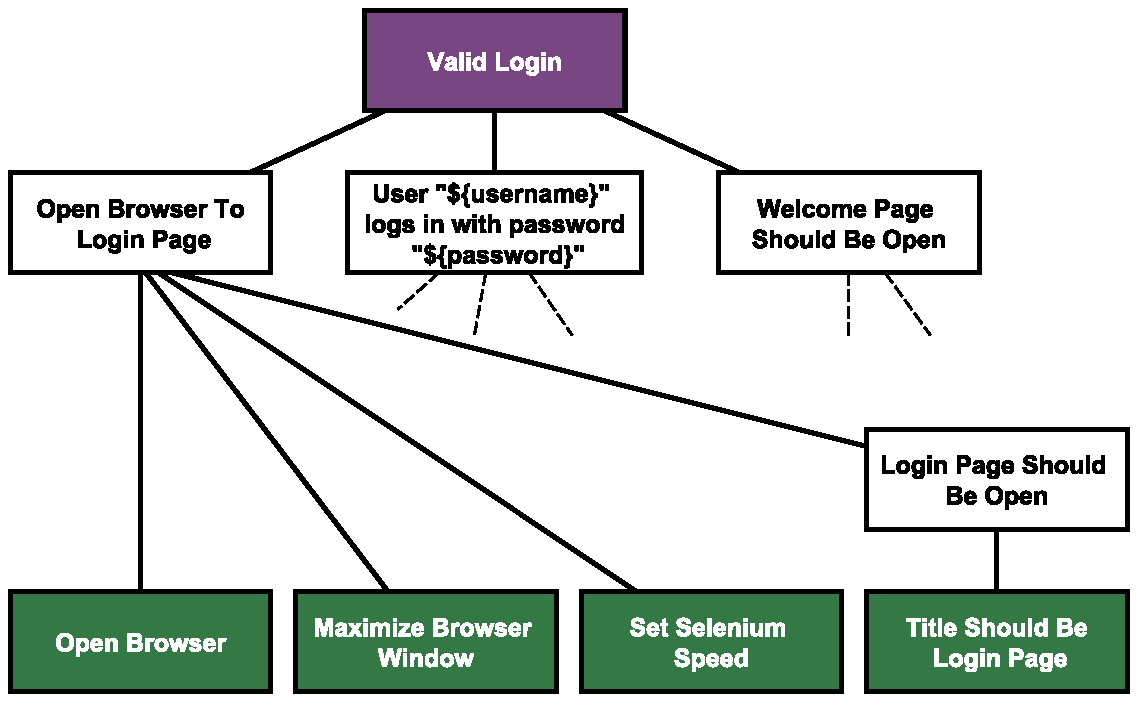
\includegraphics[width=0.7\columnwidth]{figures/evolution/robotframework_tree.pdf}
\caption{Tree representation of the ``Valid Login'' KDT test.}
\label{fig:robotframework_tree}
\end{figure}

We group keywords into seven categories based on their functionality and present them in Table \ref{keywords_categories}. We define a \emph{SYNC} keyword category for keywords dealing with the synchronization between tests and SUT; e.g., a keyword that waits 10 seconds for a GUI element of the SUT to become available. In the rest of the paper we use the term keyword to refer to \emph{User Keywords} unless stated otherwise.

\begin{table}
\caption{Keyword categories}
\label{keywords_categories}
\centering
\begin{tabular}{>{\raggedright}m{0.9in}>{\raggedright}m{4in}}
\toprule
\textbf{\scriptsize{Label}} & \textbf{\scriptsize{Explanation}}\tabularnewline
\toprule

\scriptsize{\textit{ACTION}} & \scriptsize{Keyword performing an action on the
SUT capable of modifying its state.} \tabularnewline

\scriptsize{\textit{ASSERTION}} & \scriptsize{Keyword verifying that a predicate
is true at a specific point of test execution} \tabularnewline

\scriptsize{CONTROLFOW} & \scriptsize{Keyword allowing to modify the
                                   control flow of the test execution.} \tabularnewline

\scriptsize{GETTER} & \scriptsize{Keyword allowing to extract an element from
the SUT.} \tabularnewline

\scriptsize{LOGGING} & \scriptsize{Keyword dumping logs during execution.}
\tabularnewline

\scriptsize{SYNC} & \scriptsize{Keyword relating to the
                                  synchronization between the SUT and the tests.} \tabularnewline

\scriptsize{\textit{USER}} & \scriptsize{Keyword created by a user.}
\tabularnewline

\bottomrule
\end{tabular}
\end{table}


One the tools used for the application of KDT is Robot Framework \cite{RobotFramework2020}. Robot Framework is a popular framework used world-wide by major companies, including Nokia, KONE, ABB. This is also the tool adopted by our industrial partner and, thus, used in this work. Robot Framework is an open source tool originally developed by Nokia Networks and is mainly used for acceptance testing. The ``Valid Login'' KDT test of Listing~\ref{lst:robot} was written using this framework.

One of the main advantages of Robot Framework is its high modularity.  Indeed, Robot Framework is platform-agnostic and thanks to its driver plugin architecture, the core framework does not require any knowledge of the SUT. For instance, in Listing~\ref{lst:robot}, lines 1--2 show that the script is using the external library for Selenium to interact with the SUT. Another advantage of the framework lies in its simple syntax, which makes it easily accessible to testers, regardless of their background.

\subsection{Industrial Context}
\label{sec:evolution-introduction-data}

In this work, we aim at investigating the evolution of KDT test suites at the acceptance testing level based on the industrial practice. To this end, we work together with BGL BNP Paribas that has recently (1 year ago) adopted KDT and uses it in its daily software development work for acceptance testing.

One of the reasons that our partner adopted KDT is that test cases at this testing level were created by different domain experts (business analysts and automation experts) and the adoption of a common language between the experts was imperative. All the tests used in our study have been created by a team of 3 testers and 2 business analysts working at BGL BNP Paribas using Robot Framework.

The project used in our study, hereafter referred to as \emph{SubjectA} for confidentiality reasons, pertains to all the business activities of our partner. The front-end is a web application implemented in AngularJS, and, the back-end is composed of hundreds of services written in various programming languages. These services are managed by different teams, involving more than 100 developers. The KDT test suite used in our study, referred to as \emph{TestSuiteA}, is developed by 3 testers working at the Quality Assurance (QA) team of our partner and 2 business analysts.

\begin{figure}[t!]
  \centering
  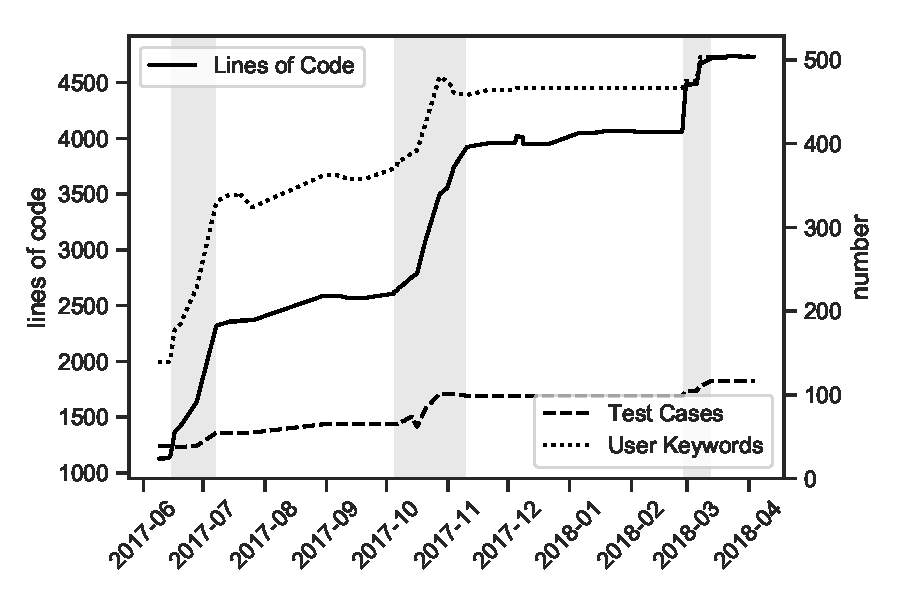
\includegraphics[width=0.7\columnwidth]{figures/evolution/project_evolution.pdf}
  \caption{Evolution of TestSuiteA}
  \label{fig:project_evolution}%\setlength{\tabcolsep}{5.1px} 
\end{figure}

Figure~\ref{fig:project_evolution} shows the evolution of TestSuiteA across the eight-month period studied. The figure depicts the evolution of the number of \emph{Test Cases} comprising the test suite, the number of \emph{User Keywords} and the lines of code of the test suite. As can be seen, our analysis begins with a test suite of 39 test cases, 139 user keywords and 1129 lines of code and ends with 117 test cases, 505 keywords and 4732 lines of code.

In the time span depicted in Figure~\ref{fig:project_evolution}, we isolated three periods during which we saw an increased test creation activity (shown in grey). After discussing with the QA team, they corroborated that these periods were more focused on test creation and the remaining ones on test maintenance. Thus, we analyze separately these periods (greyed and non-greyed) and refer to them as ``Creation'' and ``Maintenance''.

\section{Research Questions}

In this study, we attempt to answer two main questions about KDT test suites at the acceptance testing level: ``\emph{What are the benefits and challenges of adopting KDT?}''  and ``\emph{What kind of changes are performed during the evolution of a KDT test suite?}''. Answers to these questions will enable practitioners to make more informed decisions about KDT and will improve our understanding of KDT test suite evolution. Thus, we pose the following research questions:

\begin{description}
\item[\textbf{RQ1}:] \emph{What types of test code changes are performed during KDT test suite evolution?}
\end{description}

Analyzing the changes performed by the testers during KDT test suite evolution forms the basis of any automated test refactoring and test repair technique. Although research presents such information in the case of unit testing \cite{Pinto2012}, no previous study has discussed such fine-grained changes in the context of KDT at the acceptance level, to the best of our
knowledge.

\begin{description}
\item[\textbf{RQ2}:] \emph{How complex are the KDT test suites and how does this complexity affect their evolution?}
\end{description}

As mentioned in Section \ref{sec:evolution-introduction}, one of the advantages of KDT is that it allows the separation of the technical implementation details of test code and its corresponding intention. This fact can lead to test suites having several ``levels of abstraction'' (cf. Figure \ref{fig:robotframework_tree}). To this day, it is not clear how complex the KDT test code is and how this complexity affects its evolution. Answering this question will provide us with a better understanding of the difficulties faced by practitioners when they try to apply KDT and can guide future research directions in ameliorating these problems.

\begin{description}
\item[\textbf{RQ3}:] \emph{Does code duplication exist in KDT test code bases? What is its impact on the evolution of the test code?}
\end{description}

Similar code fragments are known to exist in source code and test code alike \cite{Baker1995, Roy2009, Rattan2013, Lavoie2017}. In RQ3, we investigate whether KDT codebases contain duplicated test code and how these test clones affect the evolution of the test codebase. Answering this research question is important because if such test clones exist, we need to investigate appropriate techniques to detect them, analyze them and monitor their evolution.

\begin{description}
\item[\textbf{RQ4}:] \emph{What are the practitioners' perceptions of the
    benefits and challenges of KDT in practice?}
\end{description}

RQ4 pertains to documenting and analyzing the practitioners' opinion about the advantages and disadvantages of KDT. Such analysis can help other testers to adopt (or not) KDT. Additionally, this research question gives us the opportunity to ask the practitioners' opinion about our results, validating them and understanding them better.

\section{Research Protocol}

\subsection{Definitions}
\label{sec:evolution-protocol-definitions}

\begin{itemize}
    \item \textbf{Tree}: Keywords can be represented as trees, thus, we can define a $tree\; T$ as an ordered, directed, acyclic graph with nodes $N(T)$ and edges $E(T) \subseteq N(T) \times N(T)$. The nodes of the tree denote keywords and each edge between two keywords denotes a ``step'': the parent keyword has the child keyword as a \emph{step}. For instance, in Figure \ref{fig:robotframework_tree}, keyword ``Open Browser To Login Page'' has four steps: ``Open Browser'', ``Maximize Browser Window'', ``Set Selenium Speed'' and ``Login Page Should Be Open''. As the tree is ordered, the execution of the steps will follow the order in the tree, from left to right. A node with no parent is a $root$ node that should be defined in the \emph{Test Case} block,  while a node with no children is a $leaf$ node and should be a \emph{Library Keyword}.

    \item \textbf{Keyword Level}: The \emph{level} of keyword $k$, is the maximum number of edges that exist on the subpath(s) from $k$ to a leaf keyword. In Figure \ref{fig:robotframework_tree}, ``Login Page Should Be Open'' is a \emph{level 1} keyword whereas ``Open Browser To Login Page'' is a \emph{level 2}. \emph{Library Keywords} at the leaves of the tree have a \emph{level 0}.

    \item \textbf{Keyword Connectivity}: Connectivity is a metric of reusability among the keywords. A keyword can belong to several test cases represented as trees: let keyword $k$ belong to trees $T_1, T_2, ... T_n$, i.e. $k \in N(T_1) \cup N(T_2) \cup ... \cup N(T_n)$, then we calculate the connectivity of $k$ by counting the number of nodes (keywords) in the subpath(s) from the root nodes of $T_1, T_2, ... T_n$ to $k$.

    \item \textbf{Keyword Churn}: Keyword churn is the number of lines of code added, edited or deleted from one version to the next over a period of time.
\end{itemize}

The last 3 definitions correspond to metrics used in our study. The \emph{keyword level} is used to group keywords having equal levels together. According to the philosophy of KDT, lower level keywords should be more linked to the technical details of the SUT whereas higher level keywords should be more abstract, expressing the functional requirements. The \emph{ connectivity} metric expresses the degree to which a keyword is reused and, as a consequence, the degree to which a change to this keyword can impact the test suite. Finally, the \emph{churn} corresponds to the degree to which a keyword is changed during the evolution of the test suite.

\subsection{Answering RQ1}
\label{sec:evolution-protocol-rq1}

To answer RQ1, we extract all the changes occurring in the test suite and group them per type of change. The types identified describe an action (insert, update, delete) performed on a code unit element (\emph{User Keyword}, \emph{Test Case}, \emph{Variable}, etc.). 

To this end, we extracted the 129 commits from the evolution of TestSuiteA. For each pair of consecutive commits, we gather the changes using a fine grain change algorithm.

The algorithm relies on previous, state-of-the-art studies \cite{Chawathe1996, Falleri2014, Fluri2007, Pinto2012}. In these studies, the authors built abstract syntax trees (ASTs) of Java classes and used tree edit distance algorithms to extract an optimal change path from one tree to the other, with each tree corresponding to a version of the code base.

To detect the changes, the algorithm works in two phases:

\begin{enumerate}
    \item Finding a match between elements of $v_1 \in V$ and $v_2 \in V$ where $V$ is the set of versions -- with one version corresponding to one commit -- to come up with a mapping $e_{1n} \rightarrow e_{2n}$ where $e_{mn} \in E_n$ and $E_n$ is the set of elements from $v_n$.
  
    \item Finding a minimum edit script that transforms $V_1$ to $V_2$ given the computed mapping.
\end{enumerate}

Phase 1 is essential to the edit script since the more elements that can be matched, the better the minimum edit script will perform. Phase 2 produces  an edit script detecting the basic edit operations \emph{INSERT}, \emph{UPDATE}, \emph{DELETE} for each pair of matched elements.

\begin{algorithm}[!t]
\caption{Element Matcher}
\label{alg:element_matcher}
\begin{algorithmic}[1] 
\REQUIRE $E_1 \subset v_n$, $E_2 \subset v_{n+1}$
\ENSURE final matching set: $M_{final}$
\STATE $M_{final} \leftarrow \emptyset$
\STATE $E_{1,unmatched} \leftarrow \emptyset$
\FOR{$e_1 \in E_1$}
\IF{$findMatchFileAndName(e_1,E_2)$}
\STATE $M_{final} \leftarrow M_{final} \cup (e_1,e_2)$
\STATE $E_2 \leftarrow E_2 - e_2$
\ELSE
\STATE $E_{1,unmatched} \leftarrow E_{1,unmatched} \cup e_1$
\ENDIF
\ENDFOR
\FOR{$e_1 \in E_{1,unmatched}$}
\IF{$findMatchFileAndContent(e_1,E_2)$}
\STATE $M_{final} \leftarrow M_{final} \cup (e_1,e_2)$
\STATE $E_2 \leftarrow E_2 - e_2$
\ELSIF{$findMatchNameAndContent(e_1,E_2)$}
\STATE $M_{final} \leftarrow M_{final} \cup (e_1,e_2)$
\STATE $E_2 \leftarrow E_2 - e_2$
\ELSE
\STATE $M_{final} \leftarrow M_{final} \cup (e_1,\emptyset)$
\ENDIF
\ENDFOR
\FOR{$e_2 \in E_2$}
\STATE $M_{final} \leftarrow M_{final} \cup (\emptyset, e_2)$
\ENDFOR
\end{algorithmic}
\end{algorithm}

Listing \ref{alg:element_matcher} presents the algorithm used for phase 1 to find an appropriate matching set $E_{1n} \rightarrow E_{2n}$.

\begin{itemize}
    \item \textbf{Lines 3--10}: Search for two elements present in the same file with the same name. If no match is found from $e_1 \in E_1$, it is tagged as unmatched.

  \item \textbf{Lines 11--21}:  The same operation is performed, relaxing the constraints. First, at line 12 the name is relaxed, to check if the element was renamed. Then at line 15 the file is relaxed to check if the element was moved to another file. If no suitable match is found for $e_1 \in E_1$, it is matched with a $null$ element and will be consider as a \emph{DELETE} operation in phase 2.

\item \textbf{Lines 22--24}: Check if there are elements from $E_2$ that weren't matched, in which case they will be considered as an \emph{INSERT} operation in phase 2.
\end{itemize}

In phase 2, for each pair of matched elements, we extract the differences. In the case of \emph{User Keyword} and \emph{Test Case}, we use an edit distance algorithm on the sequence of steps which is a modification of the \emph{String-to-String} algorithm presented in \cite{Ukkonen1985} using the Levenshtein edit distance.

\subsection{Answering RQ2}
\label{sec:evolution-protocol-rq2}

For each keyword we extract its level and connectivity, using the tree structure of KDT presented in Section~\ref{sec:evolution-protocol-definitions}. We then cluster the keywords by each of these metrics. For each group, we analyze the number of changes performed and the keyword churn. In order to avoid skewing the churn results, we compute the churn during ``Creation'' and ``Maintenance'' separately.

Next, we attempt to provide an estimation of the number of changes saved due to the reusability offered by KDT. To answer this, for each tests, we create a sequence of steps executed during execution. Therefore, if a keyword is used twice, the steps from that keyword would appear twice in the sequence. We then compute the changes for each sequence of step execution from one version to the next. The sequences of steps obtained are similar to the ones generated by a classical Capture/Replay (CR) tool. While these results cannot be used to directly compare the maintenance cost of CR and KDT, it provides an estimation of the benefits of reusing keywords.

\subsection{Answering RQ3}
\label{sec:evolution-protocol-rq3}

To answer this question, we extract similar keywords, also referred to as clones in the literature, and we analyze their evolution. To detect test clones in KDT test suites, we built a clone detection tool specifically designed for KDT test code. The tool is based on the fine grain change algorithm presented in the previous section. We extract the differences between each pair of keywords $k_1, k_2 \in E_n$, ignoring changes related to documentation and \emph{update name} (cf. Table~\ref{table:total_changes}).  For each pair $k_1, k_2$ we check whether they belong to one of the two types of clones analyzed in our work (definitions adopted from \cite{Lavoie2017}):

\begin{itemize}
    \item \textbf{Type I keyword clones}: identical keywords except for changes in white space, layout and documentation. The clone detection tool tags a keyword pair as Type I clones only in the case of an empty set of differences.
  
    \item \textbf{Type II keyword clones}: keywords with a content syntactically  identical except for step arguments. The clone detection tool tags a pair as Type II clones only if the set contains differences of type \emph{update step arguments} and/or \emph{update step return values} from Table~\ref{table:total_changes}.
\end{itemize}

 Additionally, for each keyword, we extract the set of changes happening during the period under study. From this change list, we define 3 types of keyword evolution:
 
 \begin{itemize}
   \item \textbf{Keyword evolving}: If the change list of a keyword $k$ is not empty, it is defined as evolving.
   
   \item \textbf{Keyword co-evolving}: Among the set of keywords evolving, keywords $k_1, k_2$ are defined as co-evolving if their changed list is identical.
   
   \item \textbf{Keyword not evolving}: Keyword $k$ is defined as not evolving if its change list is empty. 
 \end{itemize}

 Finally, we analyze the relationship between keyword evolution and keyword similarity by cross analysis of categories.

\section{Experimental Results}
\label{sec:evolution-results}

\subsection{RQ1: Types of Changes during KDT  Test Suite Evolution}
\label{sec:evolution-results-rq1}

This research question pertains to the types of changes performed by the testers during TestSuiteA evolution. The identified types and their total amount are presented in Table~\ref{table:total_changes}. The first column of the table shows the type of changes as extracted by our change algorithm. The next columns present the total amount of these changes during the \emph{Creation} and \emph{Maintenance} periods (as defined in Section \ref{sec:evolution-introduction-data}) over the 8 months of the study.

\begin{table}
\caption{Types and total amount of changes over the 8-months study}
\label{table:total_changes}
\centering
\begin{tabular}{lrr}
\toprule
change type &  Creation &  Maintenance \\
\midrule
insert documentation          &       \textbf{430} &            2 \\
insert step                   &       135 &           62 \\
insert test case              &        94 &           12 \\
insert user keyword           &       394 &           80 \\
insert variable               &       286 &           77 \\
update documentation       &       106 &           96 \\
update for loop body       &         0 &            0 \\
update for loop condition  &         0 &            0 \\
update name                &        45 &            6 \\
update step                &       249 &          107 \\
update step arguments      &       105 &          \textbf{144} \\
update step expression     &         7 &            6 \\
update step return values  &         0 &            1 \\
update step type           &         5 &            3 \\
update variable definition &        34 &           45 \\
delete documentation       &         0 &            2 \\
delete step                &        25 &           34 \\
delete test case           &        26 &            2 \\
delete user keyword        &        70 &           38 \\
delete variable            &         6 &           23 \\
\midrule
Total                      &      2017 &          738 \\
\bottomrule
\end{tabular}
\end{table}

We see that during \emph{Creation}, the main activities in terms of number of changes is ``insert documentation'', ``insert user keyword'', ``insert variable'' and ``update step''. The first three types of changes are naturally related to test creation, so this outcome is expected. A more interesting finding is that a lot of effort is devoted in documenting the keywords created. After discussing with the QA team, this effort is justified by the fact that this documentation will prove useful in the case of KDT test failures. ``Update step'' refers to modifications of steps of existing keywords. The specific kinds of modifications will be further investigated later in the section (see also Figure \ref{fig:changes_steps}).
  
\begin{figure}
\centering
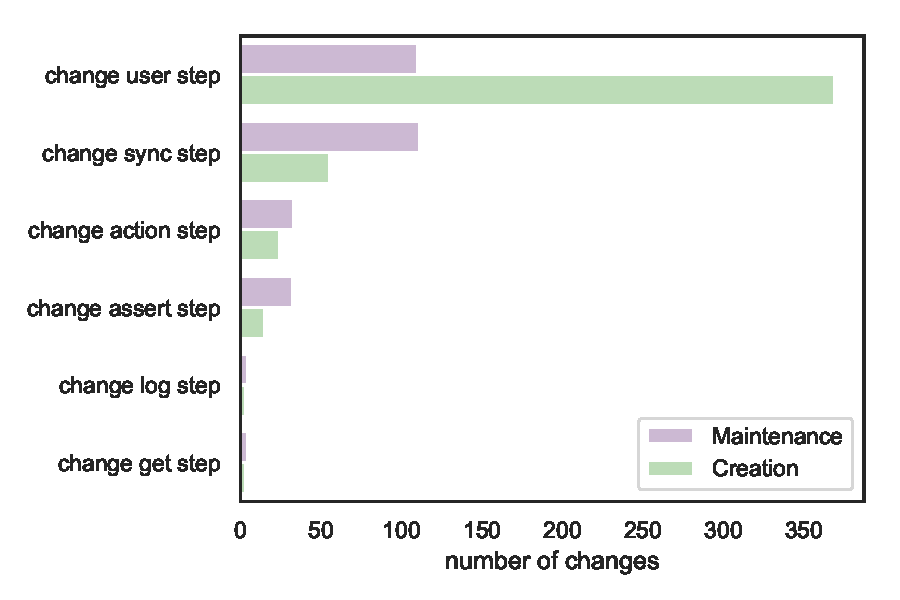
\includegraphics[width=0.7\columnwidth]{figures/evolution/changes_categories.pdf}
\caption{Total number of step changes per type}  
\label{fig:changes_steps}
\end{figure}

During \emph{Maintenance}, the main types of changes performed are the ``update step arguments'', the ``update step'', ``update documentation'' and ``insert user keyword''. After manually analyzing the changes to the arguments, we found two prevalent categories of commonly-changed arguments: arguments referring to \emph{synchronization} between the SUT and the KDT tests, e.g. wait 3 seconds and arguments referring to \emph{locators}, i.e., ways of locating elements in the GUI interface of the SUT. The arguments of the first category are typically used in the \emph{SYNC} category of Table \ref{keywords_categories}, and the latter at keywords of the \emph{ACTION} and \emph{ASSERTION} categories. Our results suggest that keywords belonging to these categories experience a high number of changes. Practitioners corroborate those results and motivate those results in RQ4.

\begin{figure}
\centering
\subfloat[Keyword Level \label{fig:boxplot_depth}]
    {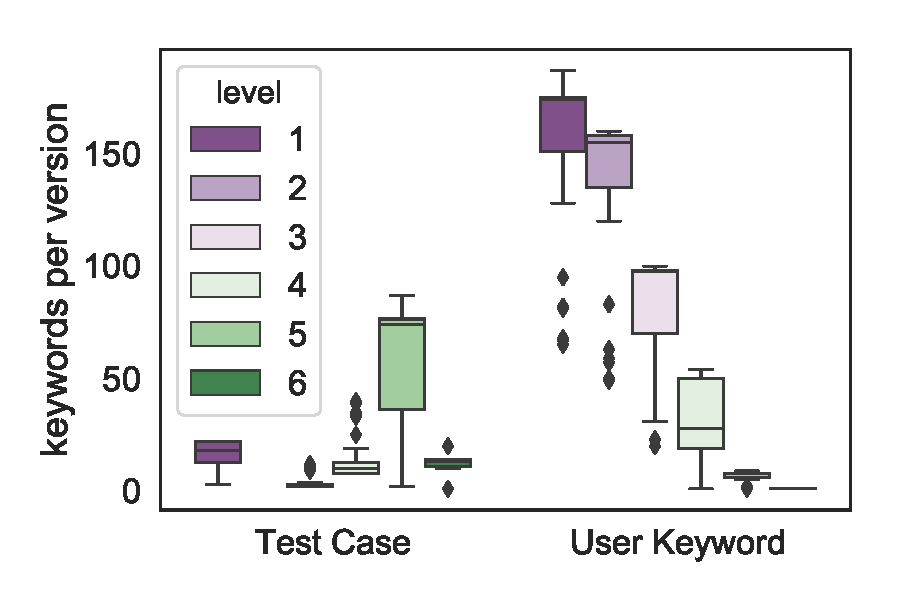
\includegraphics[width=0.7\textwidth]{figures/evolution/boxplot_depth.pdf}}
\subfloat[Keyword Connectivity\label{fig:boxplot_connectivity}]
    {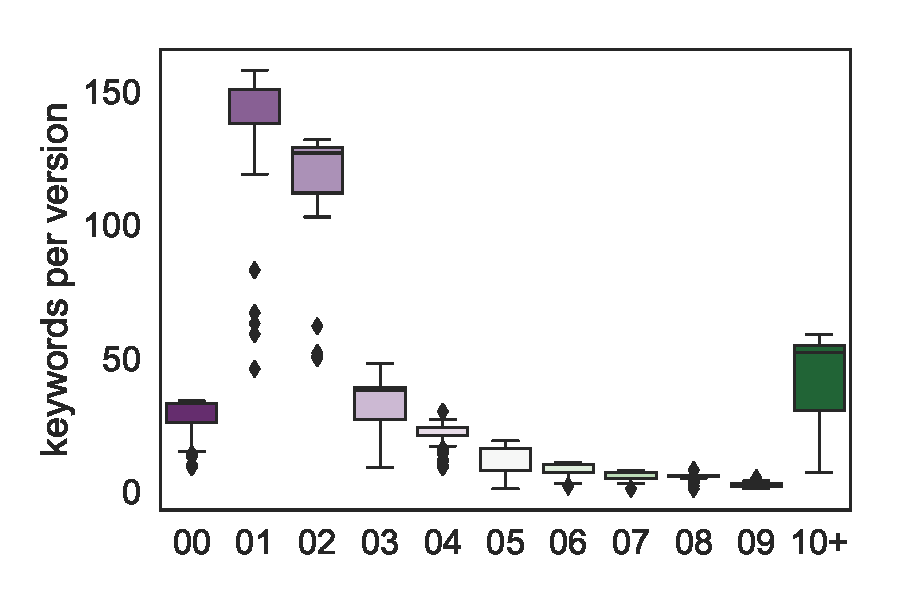
\includegraphics[width=0.7\textwidth]{figures/evolution/boxplot_connectivity.pdf}}
\subfloat[Connectivity per level category \label{fig:boxplot_depth_connectivity}]
    {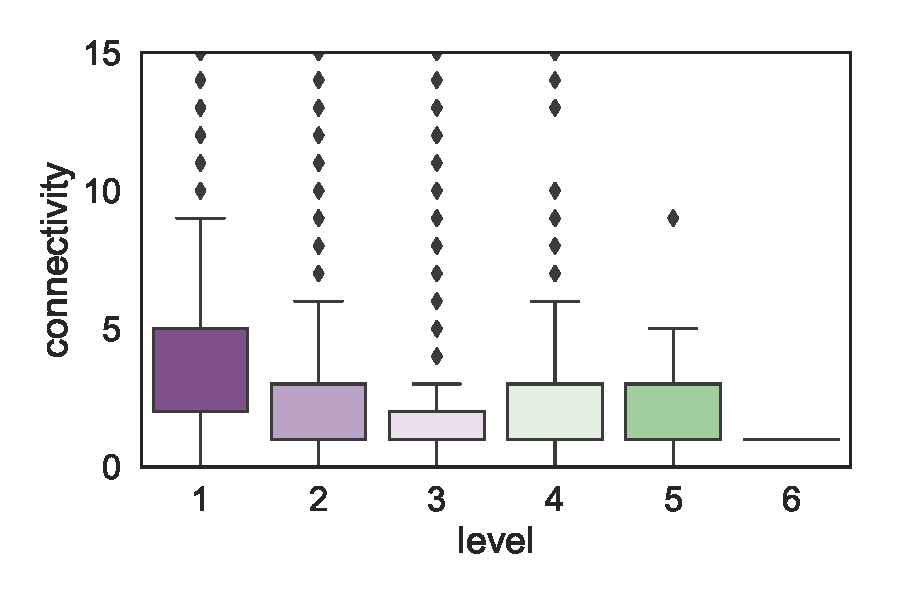
\includegraphics[width=0.7\textwidth]{figures/evolution/boxplot_depth_connectivity.pdf}}
\caption{Understanding KDT Test Suite Complexity}  
\label{fig:code_metrics}
\end{figure}

% susceptible to changes easily. The problem of defining \emph{locators} robust
% to changes has already been explored in the literature
% \cite{leotta_ICST_2015}.

Apart from ``update step arguments'', ``update step'' constitutes one of the most common change for both \emph{Creation} and \emph{Maintenance} periods. To further investigate the nature of these changes, Figure~\ref{fig:changes_steps} plots the number of changes (x-axis) against the category of the enclosing keywords (y-axis), as presented in Table~\ref{keywords_categories} with different colors for the periods studied.

As can be seen from the figure, \emph{change user steps} is by far the greatest activity during creation, we see that changes in \emph{synchronization steps} are equally important during maintenance. The interview conducted in RQ4 motivate that finding and explains it by the fact that many keywords are refactored during creation of new tests to become more generic so they can be reused. Another trend is that except for the \emph{user steps}, all other categories evolve more during maintenance. This is due to the same effect as mentioned earlier where changes in the application cause tests to break. \emph{user steps} are less affected by that effect since they are more abstract and thus less sensitive to trivial application evolution.

\subsection{RQ2: KDT Test Suite Complexity and Evolution}
\label{sec:evolution-results-rq2}

The results for RQ2 are split into two parts: first, results about the complexity of KDT test suites are reported; and, second, the way this complexity affects its evolution is presented.

\subsubsection{KDT test suite complexity}
\label{sec:kdt-test-suite}

To understand KDT test suite complexity, we calculate the \emph{keyword level} and \emph{connectivity} metrics, defined in Section~\ref{sec:evolution-protocol-definitions}. The first metric refers to the different ``abstraction levels'' (moving from pure technical to requirements expression) of the test suite and the second one, to the reusability among the keywords. Figures \ref{fig:boxplot_depth} and \ref{fig:boxplot_connectivity} present the corresponding results.

Figure~\ref{fig:boxplot_depth} depicts our results of the \emph{keyword level} for \emph{Test Cases} and \emph{User Keywords}, with the y-axis referring to the number of keywords per version. Recall that \emph{Test Cases} are the complete instantiation of a test - root node in the tree representation - and \emph{User Keywords} are user defined abstraction of the steps - intermediate nodes in the tree representation - (see also Section~\ref{sec:introduction-test-scripting}). As can be seen from the figure, most \emph{Tests Cases} are relatively complex, with a level of 5, whereas most \emph{User Keywords} are simple (levels 1 to 2). This indicates that most user defined actions remain simple, in accordance with the philosophy of KDT.

Regarding the keyword reusability, Figure~\ref{fig:boxplot_connectivity} plots the number of keywords per version (y-axis) with the \emph{keyword connectivity} (x-axis). As can be seen, there is a high degree of reusability among \emph{User Keywords}. More precisely, only 20.34\% of the lines of code are used only once. Overall, the reused keywords amount to 51.56\% of the total lines of code of TestSuiteA. As we will see next, this reusability is key to the decreased cost of the KDT test suite maintenance.

Another interesting finding is the presence of dead test code, i.e., keywords not used anywhere in TestSuiteA; these keywords have a connectivity of 0 in Figure \ref{fig:boxplot_connectivity}. In total, 5.58\% of the keywords were not used, which amounts to 4.58\% of the test code base. When we presented our findings to the QA team, they were surprised and confirmed the existence of dead code, explaining that there is no tooling to support such analysis. Our tool solves this issue and it is planned to be integrated into the team's test code development processes.

To investigate whether keywords of a particular level tend to be more reused than others, Figure~\ref{fig:boxplot_depth_connectivity} plots the keyword connectivity among the different keyword levels. By examining the figure, it becomes clear that keywords levels exhibit relatively high connectivity, indicating that the reusability of keywords is not restricted to a particular level with the exception of level 1 showing a slightly higher connectivity.


% Manual analysis showed that this is due to the fact that different \emph{User
% Keywords} were created for different features of the software, therefore
% limiting reusability.

\subsubsection{KDT complexity and evolution}
\label{sec:kdt-compl-evol}

The second part of RQ2 refers to the evolution of KDT test suites and how their complexity affects it. To better understand the amount of changes performed during test code evolution, Figure~\ref{fig:churn} presents the test code churn (y-axis) over the eight-month period analyzed (x-axis), with a similar setup to Figure \ref{fig:project_evolution}.

The purple line in the figure denotes the average churn across TestSuiteA's evolution and the light purple, its variance represented here by the standard deviation. From the figure, it can be observed that during \emph{Creation}, the churn is 8.13\%, on average, whereas in the \emph{Maintenance} period, its value is 3.61\%. Overall, keywords are changed with a churn rate of 5.11\%. This number suggests that keywords are not entirely rewritten, but localized modifications are performed.

\begin{figure}
\centering
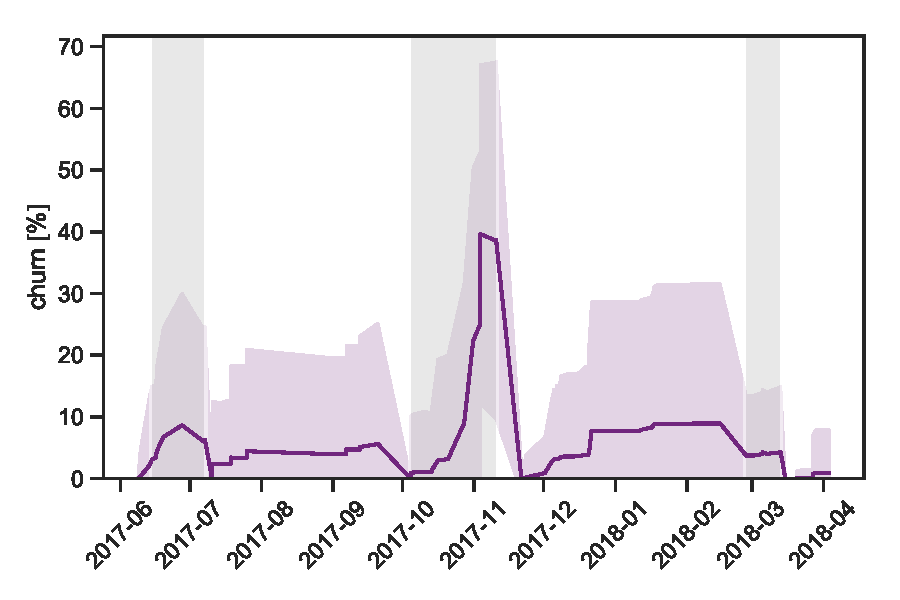
\includegraphics[width=0.7\columnwidth]{figures/evolution/time_series_churn.pdf}
\caption{KDT test code evolution: Churn over time}  
\label{fig:churn}
\end{figure}

To investigate further how the complexity of the KDT test code affects its evolution, Figure~\ref{fig:changes} plots the number of changes, for the whole period studied, against the keyword connectivity and level and Figure~\ref{fig:churn:analysis} plots the churn against the same metrics.

After examining Figure~\ref{fig:changes_connectivity}, it becomes clear that keyword reused one to three times are mostly changed. Keywords with higher connectivity do not change that often. Moreover, the figure shows that changes are performed on dead code (connectivity 0). This confirms that testers are unware of the fact that these keywords are never executed, generating easy to avoid maintenance. Regarding the results for changes and level, depicted in Figure~\ref{fig:changes_depth}, we can observe that the changes to \emph{Test Cases} do not follow a specific trend, whereas for the changes to the \emph{Users Keywords}, the lower level the keyword is, the more it is suceptible to be changed.

\begin{figure}
\centering
\subfloat[Connectivity \label{fig:changes_connectivity}]{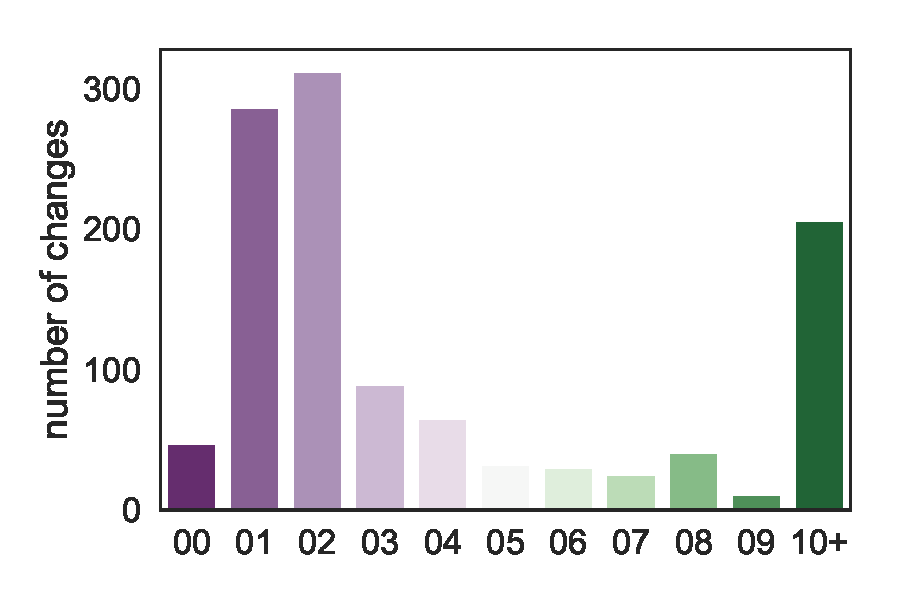
\includegraphics[width=0.7\textwidth]{figures/evolution/changes_connectivity_class_total.pdf}}
\subfloat[Level \label{fig:changes_depth}]{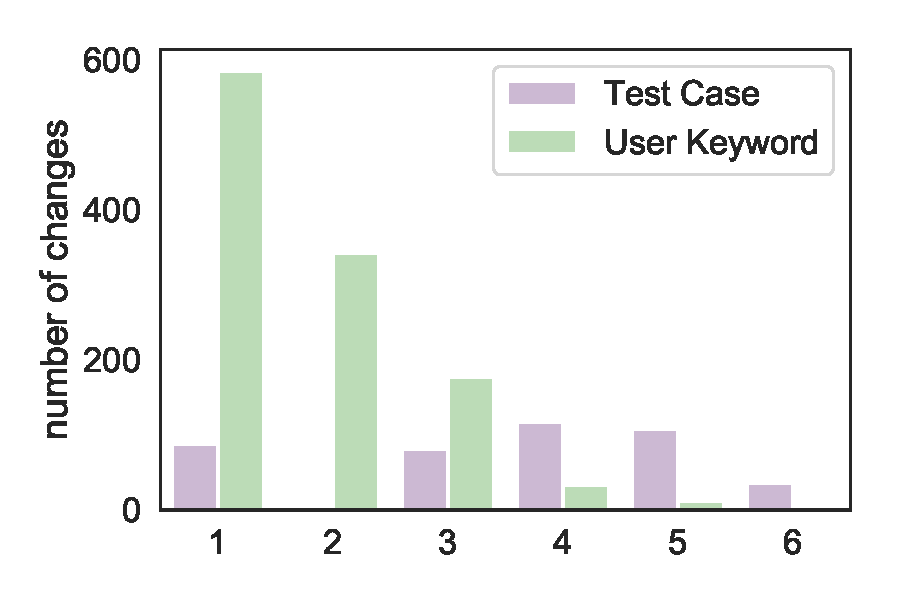
\includegraphics[width=0.7\textwidth]{figures/evolution/changes_depth_total.pdf}}
\caption{Changes distribution according to level and connectivity}  
\label{fig:changes}%\setlength{\tabcolsep}{5.1px} 
\end{figure}

\begin{figure}
\centering
\subfloat[Connectivity \label{fig:churn_connectivity}]{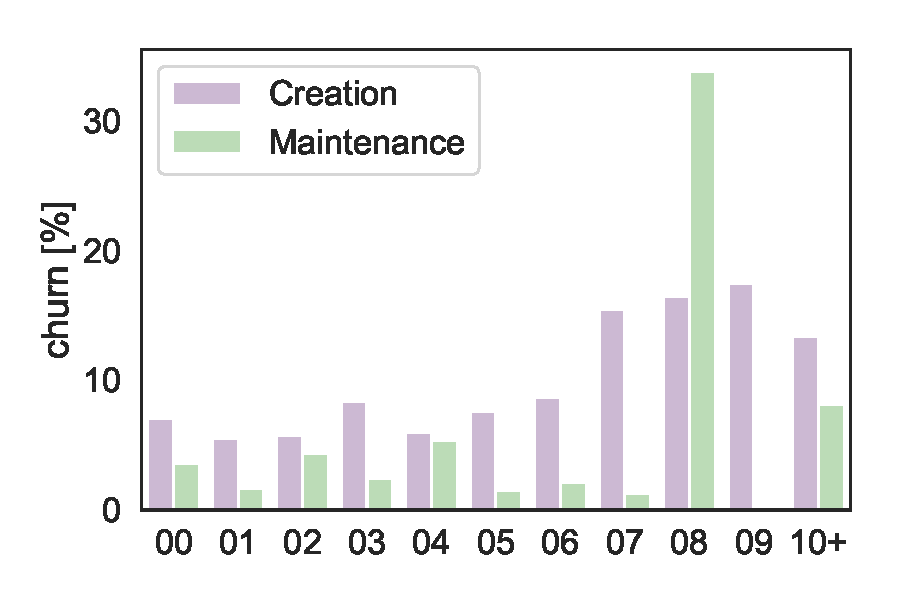
\includegraphics[width=0.7\textwidth]{figures/evolution/barplot_connectivity_class_churn.pdf}}
\subfloat[Level \label{fig:churn_depth}]{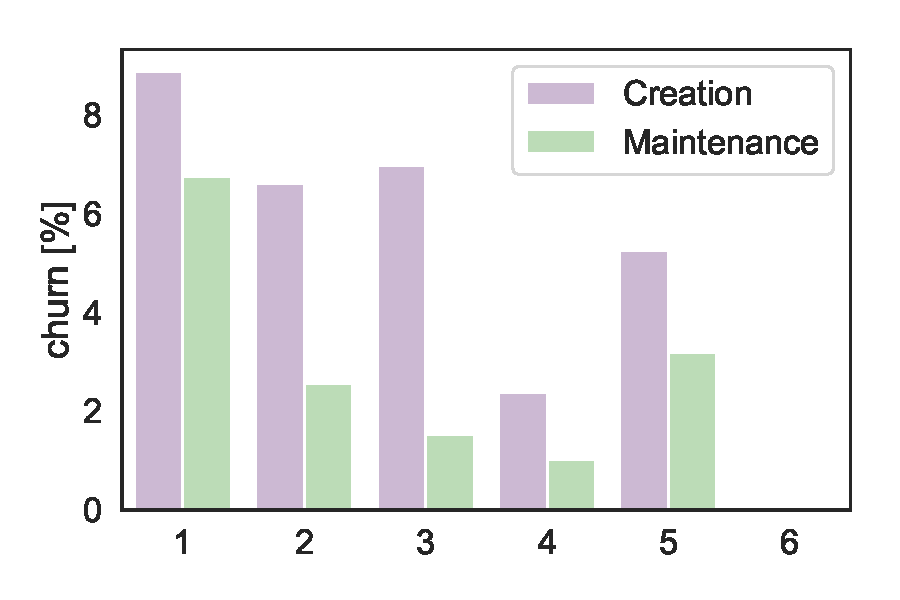
\includegraphics[width=0.7\textwidth]{figures/evolution/barplot_depth_churn.pdf}}
\caption{Churn distribution according to level and connectivity}  
\label{fig:churn:analysis}%\setlength{\tabcolsep}{5.1px} 
\end{figure}

Regarding our findings on the relation between churn rate and connectivity, depicted in Figure~\ref{fig:churn_connectivity} for the \emph{Creation} and \emph{Maintenance periods}, we can conclude that, during \emph{Creation}, keywords that are reused often, i.e. higher connectivity, exhibit approximately 50\%-60\% increased churn rate, whereas, during \emph{Maintenance} the opposite holds. Finally, regarding the results presented in Figure~\ref{fig:churn_depth} about churn and keyword level, we can see that, during \emph{Creation}, keywords with lower levels exhibit high churn values, whereas in \emph{Maintenance} this only holds for keywords of level 1. These results suggest that low level, highly reused keywords (basic action on the SUT), are evolving at a higher rate.

As we saw earlier, in TestSuiteA's evolution, keyword changed with a churn rate of 5.11\% but we also saw in the previous section that keywords are reused often. This raises the questions: How many changes have been saved due to the reusability of the keywords? To answer this question, we compare the the number of changes applied to TestSuiteA to the same suite without the keyword abstraction as explained in Section~\ref{sec:evolution-protocol-rq2}. We find that using KDT reduces the number of changes applied on TestSuiteA by 70.77\% during ``Creation'', by 72.69\% during ``Maintenance'' with an overall reduction during the entire period of 71.31\%. 

\subsection{RQ3: KDT, Test Clones and Evolution}
\label{sec:evolution-results-rq3}

In RQ3, we explore whether KDT test suites contain test clones and how these clones affect TestSuiteA's evolution. Table~\ref{table:co_evolution} presents the corresponding results. The table presents the total number of keywords that appear during the evolution of TestSuiteA (for all 129 versions) for each type of clone detected (first column -- Type I keyword clones, Type II and non-clones(``Others'')) and each type of evolution (second column). The types of evolution studied are the divided into three categories: keywords that are evolving strictly in the same way as others (``Co-evolution''), keywords that are evolving independently from others (``Evolution'') and keywords that do not evolve (``No change'').

We can observe several interesting findings from the table. First, we see that Type I and Type II clones comprise 30.2\% of the total amount keywords, indicating that almost one third of the test code written is duplicated. This finding highlights the fact that practitioners applying KDT will benefit from tools and techniques that can assist them in managing test clones.

Secondly, our results suggest that approximately 50\% of the Type I test clones evolve in the exact same way, indicating that the practitioners apply the same changes multiple times, wasting valuable effort. This is a high figure, especially when compared to the co-evolution of non-cloned keywords which is 4.9\%. Taking these results into consideration and the fact that almost 10\% of the keywords are evolving in the same way, it becomes obvious that automated refactoring techniques can reduce the maintenance effort of KDT test suite evolution.

\begin{table}
\caption{KDT Test Clones and Evolution}
\label{table:co_evolution}
\centering
\begin{tabular}{l|rrr|r}
  \toprule
         & \multicolumn{3}{c|}{Types of Evolution}                  \\
Keywords & Co-evolution &  Evolution &  No change &  Total          \\
\midrule
Type I  &          3526 &       3599 &        412 &   7537 (13.7\%) \\
Type II &           171 &       8462 &        491 &   9124 (16.5\%) \\  
Others  &          1888 &      33433 &       3184 &  38505 (69.8\%) \\
\midrule                                   
Total   &          5585 &      45494 &       4087 &  55166 (100\%)  \\ 
Percent &        10.1\% &     82.5\% &      7.4\% &    -            \\
\bottomrule
\end{tabular}
\end{table}

Finally, another interesting result exhibited in Table~\ref{table:co_evolution} concerns the overall evolution. We observe that only 7.4\% of the keywords are not evolving. This shows that during the TestSuiteA's evolution more than 90\% of the keywords are modified.

\subsection{RQ4: Benefits and challenges of KDT: The Practitioners' perspective}
\label{sec:evolution-results-rq4}

This research question pertains to the benefits and challenges of KDT as perceived by the practitioners. In the following, we present the main findings of our interviews grouped by the two main questions of our study:

\subsubsection{What are the benefits and challenges of adopting KDT?}

All interviewees agreed on two main benefits of KDT: the low learning curve and its simple syntax. Thanks to its syntax that is close to the natural language, new users can easily start being productive.  This syntax is also well-suited for communication purposes with teams that may have different backgrounds and expertise. The layered structure of keywords (i.e., the different keyword levels) plays an important role in facilitating this by hiding the technical details at the lower levels of the test suite and exhibiting the more business-oriented at the higher levels.

The main challenges encountered by the practitioners reside in their interaction with the SUT. Even a small evolution of the SUT can easily break the tests. Additionally, the testers discuss that finding the elements of the SUT that will be used in the tests is challenging, especially in applications where testability was not the primary concern.

\subsubsection{What kind of changes are performed on the test suite and why?}

The testers report two main reasons for the changes: SUT evolution and keyword adaptation.

Regarding the SUT evolution, the testers reported that as the SUT evolves, its components evolve as well which will cause the tests to adapt. The testers focus on two types of changes that are in according to our findings regarding RQ1 (cf. Section \ref{sec:evolution-results-rq1}): \emph{locators}, i.e., finding which GUI elements of the SUT should be used in the tests and \emph{synchronization} issues between the tests and the SUT.

Regarding keyword adaptation, the testers said that they create keywords in a ``best effort'' approach to cover the current needs. As new features of tests are developed, keywords are modified to become more generic. This fact explains the results illustrated in Figure~\ref{fig:changes_steps} where we observed many changes in \emph{user steps} during \emph{Creation}.

\section{Threats to Validity}

Threats to the external validity result from the generalization of our results outside the context of the study. Conducting the study with one industrial partner, the conclusions we draw may not be able to generalize to other companies using KDT. However, SubjectA is built using popular technologies, i.e., web frameworks and Java, which are wide-spread across the industry. Secondly and most important, this study is the first one, to the best of our knowledge, that analyzes the evolution of KDT test suites based on real-world data. Of course, this does not preclude the need for other studies to investigate further our results. Finally, another potential threat originates from the fact that we interviewed only 3 testers for RQ4.

Threats to the internal validity are due to the design of the study, potentially impacting our conclusions. The simple syntax of the test code allows for a robust model to be constructed. Our change algorithm presents some limitations: although phase 2 is based on the state of the art, it cannot detect \emph{Move} operations, resulting instead in two operations \emph{Delete} followed by an \emph{Insert}. This limitation might have influenced our results during the accounting of the number of changes. However, the rather low number of the \emph{delete step} operations (cf. Table \ref{table:total_changes}) indicates that this effect is marginal. Regarding the clone detection algorithm, as shown in \cite{Roy2009}, the rate of false-positives is known to be low for Type I and Type II clones.

Threat to construct validity result from the non suitability of the metrics used to evaluate the results. The main threat lies in the division of our work in two periods: ``Creation'' and ``Maintenance''. While empirical data motivated this separation, they lack of theoretical grounding. Further work on the test execution is needed to better motivate this decision.

\section{Conclusions}

Our results suggest that KDT test design is complex with several levels of abstraction and that this design favours reusability; more than 60\% of the keywords are reused which has the potential of reducing the changes needed during evolution up to 70\%.

Additionally, we find that keywords change with a relatively low rate (approximately 5\%) indicating that after a keyword's creation only fine-grained, localised changes are performed by the testers. Our results suggest that the most common changes to KDT tests are caused by \emph{synchronization} or element \emph{location} changes between the SUT and the test suite and to the \emph{assertions} of the tests. Our findings indicate that during evolution 90\% of the keywords evolve and that test clones exist in KDT test suites; approximately 30\% of the keywords are duplicated. Finally, we report on the practitioners' perception on the challenges and benefits of adopting KDT.
	\chapter{Smells in System User Interactive Tests}
\label{chap:smells-system-user-interactive-test}

\section{Introduction}
\section{Research Questions}
\section{Research Protocol}
\section{Experimental Results}
\section{Threats to Validity}
\section{Conclusions}
	\chapter{Towards more Robust Locators}
\label{chap:robust-locators}

\section{Introduction}
\label{sec:hpath-introduction}

In Section~\ref{sec:introduction-gui-testing}, we define a \gls{gui}-based test as a sequence of test steps where each test step consists of a triple: an action to be performed, the \gls{gui} element on which to perform the action and an optional value passed to the element. Consequently, for each step, the test has to be able to uniquely identify the \gls{gui} element it has to interact with. The literature identifies three locator strategies, \emph{i.e.}, ways to locate \gls{gui} elements in order to interact with the \gls{sut} \cite{Bosch2014, Leotta2018}. Each locator strategy is referred to according to its generation, all raising different concerns in term of fragility to SUIT evolution. 

The first-generation locators are based on screen coordinates for interacting with the application. While this technique was good for Record \& Replay, the high maintenance cost of this approach drove away most practitioners to the benefit of the two next generations.

The second-generation locators, also known as property- or DOM-based locators, rely on properties of \gls{gui} components in order to locate them. Here, each page is associated to a \gls{dom} offering a tree-like structure that can be navigated by means of XPath queries or \gls{css} selectors. Exploiting the \gls{dom} structure instead of directly targeting the rendered page leads to locators not affected by the properties of the rendering artifacts, such as screen resolution. However, \gls{css} selector and XPath share one pitfall: they rely heavily on internal properties of the elements they visit (e.g., its attributes or its position in the \gls{dom} tree and hierarchy of tree nodes). Despite being a reasonable strategy for most tasks they are used for (e.g., information retrieval, content formatting), this approach can be problematic in the case of automated \gls{gui} testing where the reliance on these attributes leaks structural details of the page that should not be present in the tests. Previous research \cite{Thummalapenta2013, Hammoudi2016} has shown that this leakage of structural details makes tests more sensitive to changes not related to the behavior of the application, resulting in test breakage.

While second-generation locators are wildly adopted in industry, a third-generation offers promising potential \cite{Alegroth2015}. This third-generation locators, adopted in \gls{vgt}, uses computer vision to locate elements through the bitmap graphics shown to the user at runtime. This technique was born as an answer to the fragility of second-generation tools generating high maintenance costs under \gls{sut} evolution. Indeed, relying on computer vision allows third-generation locators to be more flexible under structural changes. However, while this technique is more adaptive to underlying structural changes than second-generation locators, minor changes in the \gls{gui} representation (\emph{e.g} minor changes in the layout or in the color of \gls{gui} components) might break tests relying on the exact representation of GUI elements. Furthermore, relying on computer vision to identify \gls{gui} elements remains a non-trivial task, even though considerable progress have been made, notably with the use of machine learning \cite{White2019}.

Hence, while second- and third-generation locators each offer their own advantages, they both still contribute to test fragility \cite{Aldalur2017, Alegroth2018}. As mentioned in Chapter~\ref{chap:related-work}, to overcome the test fragility problem, academia has investigated two families of approaches: generate tests more robust to \gls{sut} evolution \cite{Montoto2011, Thummalapenta2013, Leotta2014, Yandrapally2014, Leotta2015, Leotta2016, Zheng2018} or automatically repair tests following breakages \cite{Choudhary2011, Stocco2018, Kirinuki2019}. In this chapter, our contribution falls in the former line of research as we present an attempt at reducing test breakages resulting from \gls{sut} evolution. 

To this end, we propose a novel second-generation locator, HPath, which is similar to the XPath specification but exploits rendering properties unique to \gls{html} documents. The practical benefits of HPath can be measured via its capability to generate more robust locators than the current second-generation techniques. The idea behind it is to prune the \gls{dom} tree by computing which elements are rendered. Hence, while the algorithm works in a similar fashion as absolute XPath to traverse the tree, it works on a rendered tree instead of the original \gls{dom}. Furthermore, the remaining nodes only keep a subset of their properties, the ones that affect the display. Hence, by this tree transformation, HPath relies on similar attributes as third-generation locators (no reliance on structural details) while keeping the advantages of second-generation locators (tree representation which is easy to traverse).

Before presenting HPath, we formally introduce each of the elements from the presentation layer of a web application which are exploited by algorithm and current approach to traverse it.

\subsection{Document Object Model}
\label{sec:hpath-introduction-DOM}

The \gls{dom} is a standard maintained by the \gls{w3c} until 2004 and then took over by the \gls{whatwg}. The goal is to provide a common \gls{api} which can be used with different languages in broad range of environments to generate well-formed \gls{xml} documents. According to the definition provided by the \gls{w3c}, the \gls{dom} defines the logical structure of documents and the way a document is accessed and manipulated. In this definition, a \emph{document} is the representation of a set of information that may be stored in diverse systems which would traditionally be described as data \cite{W3C2004}. In other words, the \gls{dom} formally defines the representation layer of web application. This property is what make the \gls{dom} an ideal target to generate locators.

\subsection{Hypertext Markup Language}
\label{sec:hpath-introduction-HTML}

\gls{html} is a standard markup language derived from the \gls{xml}. It is maintained by the \gls{whatwg} and designed to display the \gls{dom} in a web page. In its current implementation, \gls{html}5, it specifies a set of more granular content models which allow to improve support for multimedia and while maintaining good machine parsing capabilities, ease its readability by humans. The specification of HTML5 can be found in the \gls{html} Living Standard documentation \cite{WHATWG2021}. 

The \gls{html} syntax consists in a tree differentiating two types of nodes: (1) encoded marker (tags) differentiating bits of information composing the document or defining anchors for multimedia content and referred to as elements $E$ and (2) any other types of nodes, $N$, containing data\footnote{text node, CDATA section node, comment node,.} or lower level structural properties\footnote{attribute node, processing instruction node, document node, document type node.} of the document.

The root of an HTML document tree is an \emph{html} element, $e_{html}$. The standard enforces the presence of two unique elements as direct children of $e_{html}$ that can appear only once in the document: a \emph{head} element, $e_{head}$ and a \emph{body} element, $e_{body}$. $e_{body}$ is the sectioning root that represents the content of the document. With \gls{html}5 a lot of semantic has been added to children elements of $e_{body}$. In this work we follow the categories presented in the HTML elements reference \cite{MDN2020,WHATWG2021} (Table~\ref{tab:hpath-introduction-html5}).

\begin{table}
\centering
\caption{Categories of elements defined by the HTML elements references. When the scope of our category differs from the HTML element references, the original merged categories are mentioned in footnote.}
\label{tab:hpath-introduction-html5}
\begin{tabular}{>{\raggedright}m{1.3in}>{\raggedright}m{3.5in}}
\toprule
\textbf{\scriptsize{Category}} & \textbf{\scriptsize{Description}}\tabularnewline
\toprule
\scriptsize{\textit{Document Metadata}} & \scriptsize{Elements encapsulating data that are not present in the page, but rather, affects the way content is presented or provides additional information about the document. \emph{e.g.} $E_{link}$, $E_{meta}$ and $E_{style}$.} \tabularnewline
\scriptsize{\textit{Content Sectioning}} & \scriptsize{Elements providing landmark to organize the content of a document into logical pieces. According to the \gls{w3c} recommendation, the structural information conveyed visually to users should be represented programmatically by the appropriate sectioning element defined by the ARIA landmark roles\cite{W3C2014}. \emph{e.g.} $E_{aside}$, $E_{footer}$, $E_{nav}$, etc.} \tabularnewline
\scriptsize{\textit{Text Content\parnote{\scriptsize{Text Content and Table Content.}}}} & \scriptsize{Elements organizing blocks of content, typically text. \emph{e.g.} $E_{li}$, $E_{p}$, $E_{blockquote}$, etc.} \tabularnewline
\scriptsize{\textit{Inline Text Semantics\parnote{\scriptsize{Inline Text Semantics and Demarcating Edits.}}}} & \scriptsize{Elements formating text such as bold, italic, etc. There are also knowon as \emph{inline} content. \emph{e.g.} $E_{em}$, $E_{strong}$, $E_{cite}$, $E_{small}$, etc.}\tabularnewline
\scriptsize{\textit{Embedded Content\parnote{\scriptsize{Embedded Content, Image \& Multimedia, SVG \& MathML and Web Components.}}}} & \scriptsize{Elements allowing to embedded multimedia resources and other content. They provide information about where to load the content from and how to display it. \emph{e.g.} $E_{img}$, $E_{object}$, $E_{embed}$, $E_{video}$, etc.} \tabularnewline
\scriptsize{\textit{Interactive\parnote{\scriptsize{Interactive and Form.}}}} & \scriptsize{Elements with which a user can interact with. Typically it represents input elements. \emph{e.g.} $E_{input}$, $E_{button}$, etc.} \tabularnewline
\scriptsize{\textit{Scripting}} & \scriptsize{Elements allowing to integrate scripting in order to create dynamic content and Web application. \emph{e.g.} $E_{canvas}$, $E_{noscript}$ and $E_{script}$} \tabularnewline
\bottomrule
\end{tabular}
\parnotes
\end{table}

A specificity of an \gls{html} document is its focus on presentation of the data. Thus, a mechanism to apply styles and positioning to elements under the sectioning root, $e_{body}$, was introduced under the form of the \gls{css}. \gls{css} defines a set of styling rules that are to be applied to target elements described by a \gls{css} selector (see Section~\ref{sec:hpath-introduction-css-selector}).

Finally, the \gls{html} standard reserves two elements with no meaning by themselves: the div element, $e_{div}$, from the Content Sectioning category and the span element, $e_{span}$, from the Inline Text Semantics category. These two types do not hold any semantic meaning. Both these elements act as placeholders to mark up user defined semantics common to their children through the use of global attributes, \emph{e.g.} class, id or name. This specific semantics can be useful when used with styling where a subtree can be targeted by a style rule or when interacting with a script to apply some processing to a portion of the document.

\begin{figure}
\centering
\caption{Example of HTML Document}
\label{fig:html-document}
\begin{minipage}{0.8\linewidth}
\begin{lstlisting}[language=HTML]
<!DOCTYPE html>
<html>
    <head>
        <style>
        .someStyle {
          border: 5px outset red;
          text-align: center;
        }
        </style>
    </head>
    <body>
        <h1>Section Header</h1>
        <div class="someStyle">
          <p id="myTarget">Text <span style="color:red">in</span> a div.</p>
        </div>
    </body>
</html>
\end{lstlisting}
\end{minipage}
\end{figure}

Figure~\ref{fig:html-document} offers an example of a \gls{html}5 Document. Line 1 defines the type of document, here notifying the parser that the document follows the \gls{html}5 standards. The element $e_{html}$ (Line 2-17) contains to children, $e_{head}$ (Line 3-9) and $e_{body}$ (Line 11-16). Within $e_{head}$ we observe the presence of an element $e_{style}$ from the \emph{Document Metadata} category, which defines some \gls{css} properties for the document. $e_{body}$ contains two elements: $e_{h1}$ (Line 12), from the category \emph{Section Content} which is used to display a title, and $e_{div}$ (Line 13-15) which does have any semantic in itself but is used to apply the style defined in the $e_{style}$ thanks to its \texttt{class} attribute (``someStyle''). Within $e_{h1}$, we observe the presence of text node, $n_{text}$ (``Section Header''). Similarly, $e_{span}$ (Line 14) applies some style to the text within it (``in'') but in this case the style is directly provided by the attribute \texttt{style}.

\subsection{DOM-based Locators}
\label{sec:hpath-introduction-locators}

A DOM-based locator can be defined as a query language for selecting a subset of targeted nodes $N_{target} \subseteq N_D$ where $N_D$ is the set of nodes contained in the document $D$. Hence, a DOM-based locator is query on a tree $D$ returning a set of nodes $N_{target} \subseteq N_D$ where the size $|N_{target}|$ varies between 0 and $|N_D|$. The \gls{html} standard describes two ways of querying a set of nodes $N_{target} \subseteq N_D$ in a \gls{html} document: XPath and \gls{css} Selector. 

\subsubsection{XPath}
\label{sec:hpath-introduction-xpath}

XML Path Language also known as XPath came from an effort to provide a common syntax and semantics to identify parts of an XML document\cite{W3C2016}. Thus, the query language is not bounded to \gls{html} document but rather to any \gls{xml} compliant document\footnote{Note that the \gls{w3c} describes a slightly modified version of the XPath 1.0 standard to interact with HTML documents.}. To query $N_{target}$, XPath relies on the concept of location path. A location path\cite{Gottlob2002} is a series of successive steps traversing the XML tree to uniquely identify of subset of its node. Thus the location path is a query expression to identify specific nodes from a tree. In the work we use both location path and query expression interchangeably.

At each step, a set of nodes, referred to as context nodes, are uniquely identified. The direct left step of the context node describe the parent node and the right step describes child nodes. During the evaluation of a context node, predicates allow to filter subset of nodes among their siblings (\emph{e.g.} all nodes with a specific attribute). Hence during the location path resolution, the path is traversed from left to right, filtering out part of the tree until it reaches the right-most step and returns the result of the query. If the left-most step is the root of the tree, we call it an absolute XPath, otherwise, if the left-most step describes the root of one or many subtrees in the document, it is said to be a relative XPath. 

Each step can be defined by a selection node criteria, an optional axis relation and an optional set of predicates\cite{Barton2003}. The selection node criteria defines the element tag from the HTML document. An axis represents a relationship to the context node, and locates relative nodes (parent, self, attributes, preceding, etc.) in the document. The predicate is an expression contained between brackets after the node criteria allowing more fine grain selection during the evaluation of the step. Predicates can express logical expressions, arithmetic operations or string manipulations \cite{Gottlob2005}.

Going back to the example presented in Figure~\ref{fig:html-document}, lets assume that $N_{target}$ is $e_{p}$. Using an absolute XPath, the query takes the following form: \texttt{/html/body/div/p}. However, note that because $e_p$ is unique in the \gls{html} document, in this case, using a relative XPath can be easy as: \texttt{//p}. Unfortunately, the introduction of a subsequent $e_p$ in the document would change the result of the latter query which would now returns more than one node. To circumvent this limitation, let's exploit the  attribute \texttt{id} of $e_p$. Thus, by relying on this attribute, we can query the document using the following XPath: \texttt{//p[@id='myTarget']}. The last XPath can be translated to: retrieve all element from the document designating a paragraph ($e_p$) for which the value of the attribute \texttt{id} equals to the text ``myTarget''.

\subsubsection{CSS Selector}
\label{sec:hpath-introduction-css-selector}

Contrarily to XPath that relies on location paths, \gls{css} Selector is a structure that determines which elements are matched in the document tree by a pattern described by the locator. Here, the locator is a chain of one or more sequences of simple selectors separated by combinators\cite{W3C2018} represented by ">". The \gls{css} standard defines 6 types of simple selectors supported by the standard: (1) type selector, (2) universal selector, (3) attribute selector, (4) class selector, (5) ID selector and (6) pseudo-class. The type selector qualify an element based on its tag, a class selector based on the class attribute of the element and an ID selector relies on the id attribute of the element. A universal selector is a wild card character (*) allowing to match any substring. The attribute selector is a generalization of the ID selector and the class selector where the name of the attribute and its values are defined. Finally, the pseudo-class concept is introduced to permit selection based on information lying outside the HTML document or that cannot be expressed using other simple selectors (\emph{e.g.} a:visited which allows to target an anchor element, $E_a$, that has already been visited).

In the example from Figure~\ref{fig:html-document}, we can observe an \gls{css} Selector at Line 5. Indeed, \texttt{.someStyle} present in $e_{style}$ is a pattern that allows to apply the style describe in Line 6-7 to all the nodes which match it, \ie\ all nodes with a \texttt{class} attribute for which the value is equal to ``someStyle''. In the case of the example, this pattern is matched by one node, $e_{div}$ at Line 13. 

Both XPath and \gls{css} Selector rely on internal properties of the elements they target by exploiting the elements attributes (id, class, etc.) which is the cause of their limited flexibility to \gls{dom} evolution. In the following section, we present HPath aiming at alleviating this limitation of DOM-based locators.
\section{HPath}
\label{sec:hpath-hpath}

Relying on the \gls{html} standard described in section~\ref{sec:hpath-introduction-HTML}, we proposed \textsc{\gls{html} Path Language (HPath)} a new query language to locate nodes in an \gls{html} document. As its name suggests, our approach is similar to the XPath specification but tailored for \gls{html} documents. While the target is the same as the \gls{css} Selector (both targeting \gls{html} documents), our scope is different. Indeed, our query language aims at providing test automation engineers more expressive and more flexible locators for GUI-based testing. In other words, the goal of our approach is to provide locators that leak as little structural details as possible by relying on properties of the \gls{html} nodes that are rendered on the page to perform the query.

The intuition behind HPath lies in the fact that, if only rendered properties are permitted in the query, then the resulting locators should be more resilient to iso-functional structural changes. As a consequence, our approach helps to reduce \gls{gui}-based test fragility \cite{Thummalapenta2013, Hammoudi2016}. Moreover, relying on rendered properties (\eg\ the label of an input field) makes the locator (and, by extension, the test script) easier to understand as the reliance on structural properties has been minimized.

\begin{table}
\centering
\caption{BNF of HPath.}
\label{tab:hpath-hpath-grammar}
\begin{tabular}{>{\raggedright}m{0.9in}>{\raggedright}m{0.2in} >{\raggedright}m{2.8in}}
\toprule
\code{LocationPath} &\code{:=} &\code{RelLocationPath | '/' RelLocationPath?}\tabularnewline
\code{RelLocationPath} &\code{:=} &\code{'/' Step | RelLocationPath '/' Step}\tabularnewline
\code{Step} &\code{:=} &\code{NameTest Predicate?  | NodeType '(' ')'}\tabularnewline
\code{NameTest} & \code{:=} & \code{Literal}\tabularnewline
\code{Predicate} &\code{:=} &\code{'[' PredicateExpr ']'}\tabularnewline
\code{PredicateExpr} &\code{:=} &\code{Number | FunctionCall}\tabularnewline
\code{FunctionCall} &\code{:=} &\code{FunctionName '(' ')' '=' '"' Literal '"'}\tabularnewline
\code{FunctionName} & \code{:=} & \code{'label' | 'legend' | 'caption' | 'figcaption'}\tabularnewline
\code{NodeType} & \code{:=} & \code{'text'}\tabularnewline
\bottomrule
\end{tabular}
\end{table}

Table~\ref{tab:hpath-hpath-grammar} presents the grammar of HPath in \gls{bnf}. HPath is expressed as a location path composed of a series of steps (in a XPath fashion, yet using different predicates). Thus, HPath navigates in the \gls{html} documents based on the properties of the nodes it traverses. Each step comprises a \emph{NameTest}, which defines the type (tag) of the context element associated to an optional \emph{Predicate} or a node $N_D \not\in E_D$. Note that only text nodes are supported since they are the only ones being rendered on the page. \emph{Predicate} returns a boolean value filtering out parts of the tree during path traversal. HPath accepts a textual input for the resolution of the predicate (\emph{Literal}) and returns whether or not the value matches the property of the context node.

In the remaining of this section we present the properties of HPath allowing it to generate more flexible location paths. We use the notation $E_{\texttt{type}}$ to describe a set of elements of type \texttt{type}, and $e_\texttt{type}$ to refer to a specific element of such a set.

\subsection{Node traversal}
\label{sec:hpath-hpath-node-traversal}

Not all nodes in an \gls{html} document are used for rendering. Indeed, placeholders can be introduced in the \gls{dom} to make pages dynamic (animation, dragging, etc.) or to provide better readability for web robots (e.g., Search Engine Optimization). Thus, by definition, these nodes should not appear in the location path when creating flexible locators for GUI-base testing. 

Therefore, the node traversal is done on a rendering tree, generated by the HPath engine, where all elements not affecting the rendering flow are pruned out. Referring to the semantic offered by the \gls{html} standard, two types of elements, $E_{span}$ and $E_{div}$, do not hold any intrinsic semantic by themselves and act as placeholders. Indeed, if no styling is applied to these elements, they are ignored by the rendering engine\cite{Grigorik2019}. Consequently, during the tree traversal, HPath ignores any $e_{span}$ or $e_{div}$ that will not affect the rendering flow.  

Because, when performing GUI testing, the locator is computed after the processing of all styling and rendering operations. To avoid misclassifying any node as not rendered, HPath relies on the browser engine to prune any nodes not affecting the display of the page. This step leads to a new \gls{html} document which only contains rendered node $N_R \subseteq N_D$. Thus, while HPath traverses the trees in a similar fashion as absolute XPath, it does so on a different tree.

\begin{figure}
\centering
\caption{Example of HTML Document with elements that are not affecting rendering}
\label{fig:html-document-not-rendered}
\begin{minipage}{0.8\linewidth}
\begin{lstlisting}[language=HTML]
<!DOCTYPE html>
<html>
    <head>
        <style>
        .someStyle {
          border: 5px outset red;
          text-align: center;
        }
        </style>
    </head>
    <body>
        <@\textcolor{block}{<div id="for-robot">}@>
            <h1>Section Header</h1>
        <@\textcolor{block}{</div>}@>
        <div class="someStyle">
          <p id="myTarget">Text <span style="color:red">in</span> a div.</p>
        </div>
    </body>
</html>
\end{lstlisting}
\end{minipage}
\end{figure}

Figure~\ref{fig:html-document-not-rendered} shows an example of a \gls{html} document containing an element (in red) not rendered by the web engines but is in any other aspect equivalent to the one presented in Figure~\ref{fig:html-document}. In the case of HPath, both document do end up generating the same working tree. Thus, lets assume we target $e_{h1}$, using absolute XPath, the query takes the form: \texttt{/html/body/div/h1}. However, in the case of HPath, the query takes the form: \texttt{/html/body/h1}.

\subsection{Predicates}
\label{sec:hpath-hpath-predicates}

While computing predicates or any other node filtering mechanism, \gls{dom}-based locators usually rely heavily on implementation-dependent properties of the elements they visit (\emph{e.g.} id or class). However, these attributes can change without affecting the functionality of a page or any of its visible parts. For example, modifying the id of a button, if not affected by a style rule, will not have any effect on its rendering. Thus, HPath defines a few selected predicates relying on rendered properties, which can take the following forms:

\begin{itemize}
    \item \textbf{label:} Most of the interactive elements $E_{interactive}$ can be associated with a label element, $E_{label}$ to provide a textual clue about their functionality. The HTML standard defines two strategies to link those elements: (1) $e_{label}$ is a direct parent of $e_{interactive}$ or (2) $e_{label}$ is a sibling of $e_{interactive}$ where the value of the attribute \emph{for} of $e_{label}$ equals the value of the attribute \emph{id} of $e_{input}$. The \textbf{label} predicate extracts the textual content (see Section~\ref{sec:hpath-hpath-text-extraction}) of $e_{label}$ associated with the context $e_{interactive}$. An example of the two forms is provided in Figure~\ref{fig:html-document-input}. Here, the query \texttt{//input[label()='City']} retrieves both $e_{input}$.
    
\begin{figure}[h!]
\centering
\caption{Extract of HTML document exhibiting input element}
\label{fig:html-document-input}
\begin{minipage}{0.8\linewidth}
\begin{lstlisting}[language=HTML]
<form>
    <fieldset>
        <legend>Address 1</legend>
        <label for="city-1">City
            <input type="text" name="city-1" id="city-1">
        </label>
    </fieldset>
    <fieldset>
        <legend>Address 2</legend>
        <label for="city-2">City</label>
        <input type="text" name="city-2" id="city-2">
    </fieldset>
</form>
\end{lstlisting}
\end{minipage}
\end{figure}
    
    \item \textbf{legend:} Related children elements of a form element ($E_{form}$) can be grouped together through the use of fieldset element ($E_{fieldset}$). Any $e_{fieldset} \in E_{fieldset}$ can be associated with a textual value defined in a legend element, $e_{legend}$. According to the standard, if $e_{legend}$ is a direct child of $e_{fieldset}$, then it is associated to the parent $e_{fieldset}$. The \textbf{legend} predicate extracts the textual content of a $e_{legend}$ associated to the context $e_{fieldset}$. An example is provided in Figure~\ref{fig:html-document-input}. In the example, as shown above, when only relying on $e_{label}$ to select the input retrieve the two $e_{input}$. To refine the selection to the first address, the query can be expressed using $e_{legend}$ as: \texttt{//fieldset[legend()='Address 1']/input[label()='City']}.
    
    \item \textbf{caption:} Table elements, $E_{table}$, can be assigned a caption through the use of a caption element $E_{caption}$. According to the standard, if a $e_{caption}$ is a direct child of a $e_{table}$, then it is associated to the parent $e_{table}$. The \textbf{caption} predicate extracts the textual content of a $e_{caption}$ associated to the context $e_{table}$. An example is provided in Figure~\ref{fig:html-document-caption}. Here, the query \texttt{//table[caption()='Locator breakages']/tr[1]} retrieves the first row of the table. 

\begin{figure}[h!]
\centering
\caption{Extract of HTML document exhibiting caption element}
\label{fig:html-document-caption}
\begin{minipage}{0.8\linewidth}
\begin{lstlisting}[language=HTML]
<table>
    <caption>Locator breakages</caption>
    <tr>
        <td>Name</td>
        <th>HPath</th>
        <th>XPath</th>
    </tr>
</table>
\end{lstlisting}
\end{minipage}
\end{figure}

    \item \textbf{figcaption:} Figure elements, $E_{figure}$, can be assigned a caption through the use of a caption element $E_{figcaption}$. According to the standard, if $e_{figcaption}$ is a direct child of $e_{figure}$, then it is associated to the parent $e_{figure}$. The \textbf{figcaption} predicate extracts the textual content of $e_{figcaption}$ associated to the context $E_{figure}$. An example is provided in Figure~\ref{fig:html-document-figcaption}. Here, the query \texttt{//figure[caption()='Length of the Locators']/img} retrieves the image. 
    
\begin{figure}[h!]
\centering
\caption{Extract of HTML document exhibiting figcaption element}
\label{fig:html-document-figcaption}
\begin{minipage}{0.8\linewidth}
\begin{lstlisting}[language=HTML]
<figure>
    <img src="locator-length.jpg" alt="Locator Length">
    <figcaption>Length of the Locators</figcaption>
</figure>
\end{lstlisting}
\end{minipage}
\end{figure}
    
\end{itemize}

If no predicate can be generated to compute the location path, then the resulting path resembles the one that would be generated by the XPath algorithm, i.e., with only positioning predicate and no axis. However, while both expression present the same syntax in such case, the difference is that HPath does not compute the path on the actual \gls{dom} but on the pruned \gls{dom} tree (as described in Section~\ref{sec:hpath-hpath-node-traversal}).

\subsection{Content Extraction}
\label{sec:hpath-hpath-text-extraction}

In the current implementation of HPath, all predicates (except the positioning predicate) rely on textual information visible on the page. To extract the content of a text under an element, XPath extracts the content of the text node, $n_{text}$, which is a direct child of the context element. HPath goes beyond this procedure and analyzes styling information contained in the elements from the Inline Text Semantics category (see Table~\ref{tab:hpath-introduction-html5}). HPath takes advantages of this semantic and filters out any element from this category when extracting text. The resulting $n_{text}$ are then merged together to reconstruct the text that will be used by the predicates for evaluation. To query $e_input$ from Figure~\ref{fig:html-document-text}, one can write the following query: \texttt{//input[label()='City']}.

\begin{figure}[h!]
\centering
\caption{Extract of HTML document exhibiting inline text semantics elements}
\label{fig:html-document-text}
\begin{minipage}{0.8\linewidth}
\begin{lstlisting}[language=HTML]
<div>
    <label for="city-2">
        <i class="fa fa-home"><b>City</b>
    </label>
    <input type="text" name="city-2" id="city-2">
</div>
\end{lstlisting}
\end{minipage}
\end{figure}
\section{Research Questions}
\label{sec:hpath-rqs}

HPath makes the assumption that some types of web elements are typically more targeted than others by \gls{suit}s and as such some elements can be removed from the \gls{dom}. Indeed, removing text formatting and non-displayed elements while being a reasonable assumption, might remove interesting elements from the \gls{dom} tree. Thus, we validate this assumption by analyzing which categories of elements are targeted by \gls{dom}-based locators in \gls{suit}s and ask:

\begin{description} 
\item[\textbf{RQ1}:]
\emph{Which categories of elements are predominantly targeted by \gls{gui}-based test scripts?} 
\end{description} 

Next, we evaluate our new approach, HPath, and compare its ability to exploit the properties of web elements through its predicates. The goal is to measure to which extend the query expression can be compressed but also to what extent HPath can generate meaningful predicates. To put these results in perspective, we compare it against two algorithms generating XPath, namely, \emph{absolute XPath} and \emph{Robula+}. This leads to the following research question:

\begin{description} 
\item[\textbf{RQ2}:]
\emph{Which element properties are exploited by the different location path strategies?} 
\end{description} 
        
Finally, we investigate the resilience against \gls{sut} evolution of HPath. The main goal of HPath being to generate query expression resistant to minor structural change in the \gls{sut}. Thus, to assess its robustness to changes, we compare it to the two XPath generation algorithms used in RQ2 and express the final research question as follow:

\begin{description} 
\item[\textbf{RQ3}:]
\emph{What is the resilience against \gls{sut} evolution of the different strategies?} 
\end{description} 
\section{Research Protocol}
\label{sec:hpath-protocol}

This section presents the experimental setup for the case studies to answer our research questions. The goal of this chapter is to analyze the impact of using second-generation locators relying on rendered features. Thus, we rely on two main concepts: the properties of an element HPath can leverage to generate a query and its resilience to changes happening during the \gls{sut} evolution. In this study, the properties are measured by the length of the location path and the presence of predicates in any step of the location path. The resilience to change of a locator is evaluated by its propensity to avoid breakage following a change in the \gls{html} document.

\subsection{Projects Collection}
\label{sec:hpath-protocol-projects}

To select adequate projects for a case study, we mine repositories from Github, using its search \gls{api} which allows applying queries to filter the result from the Github database. Because of the restrictions of the mining process described in Section~\ref{sec:hpath-protocol-elements}, we have to isolate projects with tests written in Java and exercising the Selenium \gls{api}. Furthermore, both application code and test code need to be versioned in the same repository to be able to go back in time and run test suites for previous versions.

Moreover, because of the dynamic nature of our analysis, we need to be able to compile the projects and run them on successive versions. Unfortunately, despite our best effort, most of the projects we gathered could not be executed in our experimental setup (missing dependencies, outdated build tools). Thus, this process yields two large web-based open-source systems: OpenOLAT\footnote{https://github.com/OpenOLAT/OpenOLAT}, a web-based e-learning platform, and MISO LIMS\footnote{https://github.com/miso-lims/miso-lims}, a lab information management system designed for tracking next-generation sequencing experiments. Both projects rely on a Java backend that is communicating with a \gls{rdbms}. For the front end, both use \gls{html}, CSS, and Javascript however MISO LIMS is relying on the HTML4 standard while OpenOLAT is using the \gls{html}5 standards. Finally, both projects adopt a multi-tier architecture relying on different services working in concert.

\begin{table}
\centering
\caption{Web Applications used in our experiments. Column \emph{\#Releases} presents the number of releases collected, \emph{KLoC} is the number of thousand lines of code in the last release, \emph{\#Tests} is the rounded average number of integration tests per release and \emph{\#Locators} is the total number of locators recorded.}
\label{tab:hpath-protocol-projects}
\begin{tabular}{>{\raggedright}m{0.7in}>{\raggedleft}m{0.7in}>{\raggedleft}m{0.7in}>{\raggedleft}m{0.7in}>{\raggedleft}m{0.7in}}
\toprule
\textbf{\scriptsize{Project}} & \textbf{\scriptsize{\#Releases}} & \textbf{\scriptsize{KLoC}} & \textbf{\scriptsize{\#Tests}} & \textbf{\scriptsize{\#Locators}} \tabularnewline
\toprule
\scriptsize{\textit{OpenOLAT}} & \scriptsize{8} & \scriptsize{1308} & \scriptsize{154} & \scriptsize{216424} \tabularnewline
\scriptsize{\textit{MISO LIMS}} & \scriptsize{57} & \scriptsize{326} & \scriptsize{8} & \scriptsize{15672} \tabularnewline
\bottomrule
\end{tabular}
\end{table}

Table~\ref{tab:hpath-protocol-projects} presents some key metrics of the projects under study. The 57 versions of MISO LIMS were collected between March 2019 and November 2020 and the 8 versions of OpenOLAT span from November 2018 to August 2020. 

The low number of versions for the OpenOLAT project (8 versions) is due to the fact that earlier versions could not be compiled (Maven Plugin not supported). While both projects are quite large in terms of lines of code, we can see that the developers of the project MISO LIMS do not rely heavily on \gls{gui}-based testing, with an average number of 8 tests per version.

\begin{figure}
\centering
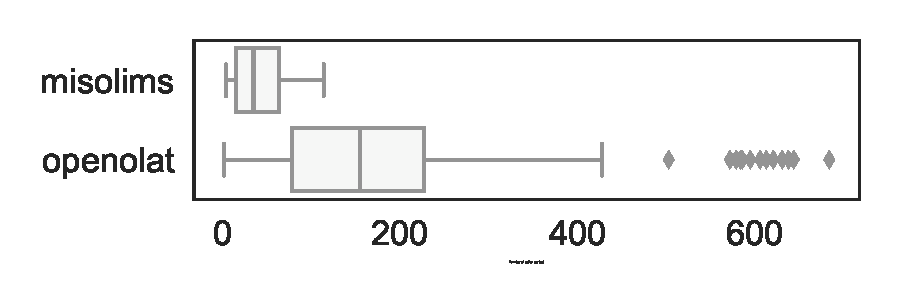
\includegraphics[width=0.8\columnwidth]{figures/hpath/selector-per-test-dist.pdf}
\caption{Number of actions triggered by test.}  
\label{fig:hpath-protocol-actions}
\end{figure}

Figure~\ref{fig:hpath-protocol-actions} presents the number of actions triggered by the tests for each project under study. In average, the number of actions triggered by a test is 170 for the OpenOLAT project and about 42 for the MISO LIMS project. One intriguing point shown by the figure is the presence of tests not containing any interaction with the application through Selenium. These are tests not targeting the \gls{sut} through the user interface but rather directly interacting with the \gls{api} of the application or the \gls{rdbms} itself, thus falling out of the purview of \gls{suit}s.

\subsection{Mining Locator Breakages}
\label{sec:hpath-protocol-elements}

We developed a tool called Mercator\footnote{Available at \url{https://github.com/UL-SnT-Serval/mercator}} to capture the state of the pages and the \gls{dom}-based locators used to interact with it in the test suites. 

\subsubsection{Selenium Instrumentation}
\label{sec:hpath-protocol-instrumention}

More specifically, Mercator instruments method calls \emph{findElement} and \emph{findElements} from the class \emph{RemoteWebDriver} offered by the Selenium \gls{api}. Hence, at runtime, Mercator captures the following data every time a test exercises a \gls{dom}-based locator: (1) information about the state of the current web page \ie\ complete dump of the \gls{dom}, size of the window and current \gls{url}; (2) information about the test \ie\ test name, call stack, inference on the previous call stack; (3) information about the locator \ie\ locator strategy, locator value; (4) information about the project \ie\ repository \gls{url}, commit id, previous commit id, commit date. This process is repeated for each version defined in the configuration of Mercator. For this study, we select every release of the projects. We restrict our study to releases because the projects rely on external dependencies which are not stable during the development cycle, thus, leading to code that cannot compile due to missing dependencies (SNAPSHOT). Furthermore, using releases increases the chances of observing genuine \gls{sut} evolution, thus, reduces noise.

\subsubsection{HTML Dump}
\label{sec:hpath-protocol-capture}

The most sensitive aspect of this process is collecting the \gls{dom} dumps. Indeed, as explained in Section~\ref{sec:hpath-introduction-HTML}, a \gls{html} document can contain links to other resources such as multimedia and \gls{css} style sheet stored externally. Thus, for the dump to be usable as a single \gls{html} document file, during the instrumentation, a complete \gls{html} document with no external dependencies needs to be computed. This is done by inlining all the \gls{css} style sheets in the header, and providing placeholders for all multimedia content retaining their attributes, size, and position. Furthermore, all properties computed by JavaScript are inlined in the style attribute of the elements, and all script elements are removed from the dump. This is possible because pages are captured after the execution of all JavaScript routines which may alter the structure of the \gls{dom} tree. Finally, comment nodes and any formatting of the \gls{html} document not affecting its content (line returns between to subsequent elements) are removed to limit syntactic differences between dumps.

One caveat encountered during instrumentation is the non-negligible amount of time (between 200ms to up to 1500ms during our experiments depending on the complexity of the page) required to create the dump. This delay causing tests to run slower might break some which are bounded by a maximum time budget (\emph{timeout}). This leads us to use a strategy to monitor changes in the \gls{dom} tree to minimize the number of times the state has to be computed. Unfortunately, these changes failed to detect changes not altering the tree but modifying external properties of the elements (mostly hovering and selections in table) which lead to generating locators in our dataset that are not valid, 20.09\% for MISO LIMS and 8.57\% for OpenOLAT. We deem this tradeoff reasonable compared to the alternative where we observe about 35\% of the tests failing due to our instrumentation.

With reasonable performance when instrumenting one version, the next step consists of devising a strategy to compute the lineage of a locator across versions. To achieve this objective, we rely on the changelog computed by the versioning system Git. Mercator enriches the data it records (locator and \gls{dom}) with information about the version and the test that is currently running. Then using the current stack trace and the changelog between the current version and the previous version (identified by their commit IDs) it is able to offer an approximation of the stack trace in the previous commit. To do so, it recomputes the stack trace in the previous version, taking into account line additions and deletions in the test code. This process is described in detail in Section~\ref{sec:hpath-protocol-pairs}.

Finally, the last step of this process is the extraction of the elements themselves. Each data point generated by Mercator contains a locator and its associated HTML document. Thus, by querying the \gls{dom} with the collected locators, we can retrieve the elements targeted by the tests relying on Selenium. The Selenium API offers different strategies to locate web elements that are shown in Table~\ref{tab:selenium_strategies}. 

\begin{table}
\centering
\caption{Element selection strategies defined by the Selenium API.}
\label{tab:selenium_strategies}
\begin{tabular}{>{\raggedright}m{1in}>{\raggedright}m{3in}}
\toprule
\textbf{\scriptsize{Strategy}} & \textbf{\scriptsize{Description}}\tabularnewline
\toprule
\scriptsize{\textit{class name}} & \scriptsize{Locates elements whose class attribute contains the search value.} \tabularnewline
\scriptsize{\textit{css selector}} & \scriptsize{Locates elements matching the CSS selector.} \tabularnewline
\scriptsize{\textit{id}} & \scriptsize{Locate elements whose id attribute matches the search value.} \tabularnewline
\scriptsize{\textit{link text}} & \scriptsize{Locates anchor elements, $E_a$, whose inner text matches the search value.} \tabularnewline
\scriptsize{\textit{patial link text}} & \scriptsize{Locates anchor elements, $E_a$, whose inner text contains the search value.} \tabularnewline
\scriptsize{\textit{tag name}} & \scriptsize{Locates elements whose tag name matches the search value.} \tabularnewline
\scriptsize{\textit{xpath}} & \scriptsize{Locates elements matching the location path.} \tabularnewline
\bottomrule
\end{tabular}
\end{table}

\subsubsection{Pairs Creation}
\label{sec:hpath-protocol-pairs}

As shown in Figure~\ref{fig:hpath-protocol-actions}, each test exercises a large number of actions, and simply relying on the test name does not offer the granularity required for this analysis. Thus, we rely on \emph{stack traces} to uniquely identify an element query in a version. The \emph{stack trace} is the stack of subroutine state information from the test entry point to Selenium API call to locate an element. Each subroutine call is defined by a fully qualified class name, a method name, and a line number. Unfortunately, this method is sensitive to changes in the test code base from one version to another. Indeed, if lines are added or deleted before the call, then the line number is affected. Furthermore, when classes or methods are renamed, the subroutine information of the corresponding frame is modified. To minimize this effect, we compute the \emph{previous stack trace} which is the stack trace that a call would have had in the previous version when accounting from the change extracted from the \emph{unified diff} obtained through the version control system. We recompute the line number based on the line additions and deletions that occurred before the call in the file. If the target line is modified or there are class or method name changes, then, we consider that no mapping is possible. At this stage, each call to Selenium API can be identified by a \emph{stack trace} and is associated with a \emph{previous stack trace}. Thus, to create the pairs we link calls qualified by a tuple $<stack\:traces,\:version>$ to calls with a matching tuple $<previous\:stack\:traces,\:previous\:version>$. We will call $version_A$ and $version_B$, the first version and the next version of the pair respectively.

\subsubsection{Breakage Detection}
\label{sec:hpath-protocol-breakage-detection}

Once the pairs are created, we filter out any pair not exhibiting a \gls{sut} evolution. For each \gls{dom} we compute a hash code based on its string representation. Then, we filter out any pair where $hash_A = hash_B$ thus only accounting for pairs containing changes in the \gls{dom}. We consider a locator to break following a change in $<DOM_A, DOM_B>$, if querying $DOM_B$ with $locator_A$ returns an empty set, \emph{i.e.} fails to locate any element. We perform this operation on all pairs of the dataset where $hash_A \neq hash_B$. This process leads to a total of 30,436 pairs.

\subsection{RQ1: Target Elements}
\label{sec:hpath-protocol-rq1}

The approach that we propose, HPath, makes the assumption that the interactions with the \gls{html} document mainly targets visible elements, \emph{i.e.} elements rendered on the web page. 

Indeed, under our hypothesis, a test should interact with elements to navigate through the states of the web application then make assertions on visible elements to validate the proper execution of the test as a human would. Thus, not all elements of the \gls{html} document hold the same value for the testers. To assess this hypothesis and answer RQ1, we extract the type (tags) of the elements targeted by the tests. Comparing this distribution with the one contained in the \gls{html} document, we can assess which elements SUITs typically interact with. 

Furthermore, previous work targets elements systematically\cite{Cohen2015, Leotta2015, Aldalur2017, Eladawy2018} or generates test scripts\cite{Grechanik2009, Montoto2011, Kirinuki2019} when a \gls{gui} test suite is not available. Unfortunately, studies relying on \emph{in vivo} \gls{gui} test suites are usually conducted on industrial projects and the source code is not available\cite{Thummalapenta2013, Yandrapally2014}. While there exists studies tackling the question of the evolution and the characteristics of \gls{gui} tests \cite{Christophe2014}, they usually rely on static analysis and do not convey information about locators and their target elements. Thus, understanding which type of elements are targeted by testers would allow researchers to create benchmarks to evaluate their approaches by following the same distributions observed in other projects when no tests are available.

\subsection{RQ2: Element Properties Used by Locators}
\label{sec:hpath-protocol-rq2}

To evaluate HPath, we compare it against two approaches to generate XPath: absolute XPath and Robula+. We select XPath algorithms because our approach is a derivative of XPath with the aim of addressing one of its limitations: its reliance on structural properties of the \gls{html} document, making HPath more flexible to changes of the internal document structure.

The first algorithm, absolute XPath, builds an XPath where each step can only rely on a positional predicate. Thus, it does not rely on any attributes such as id, class, or name and can be seen as the most naive form of XPath generation. Note that when using the absolute XPath algorithm, the deeper an element is nested in a \gls{dom} tree, the longer the location path. Thus, this algorithm tends to leak the overall structure of the \gls{dom}, where any change in the node hierarchy of target elements will alter its absolute XPath representation.

Robula+ \cite{Leotta2016} is a state-of-the-art XPath generation algorithm developed by the research community. The aim behind this algorithm is to generate robust XPath locators. It works with the assumption that the shorter the location path is, the less it leaks the overall structure of the \gls{dom}, thus making it more robust to changes in the \gls{dom} hierarchy. To generate the shortest location path possible, the algorithm starts with (\texttt{//*}), which selects every node, $N_D$, and then refine the expression in consecutive specialization steps until only the target candidate can be selected by the expression, $N_{target} \subseteq N_D$. Each refinement step is based on heuristics to improve the expressiveness and robustness of the final location path. During the refinement steps, the heuristics define the order in which Robula+ tries to select an attribute to build a predicate\footnote{We follow the recommendations from the authors: \emph{name}, \emph{class}, \emph{title}, \emph{alt}, \emph{value}.} and the attributes to ignore\footnote{We follow recommendations from the authors: \emph{href}, \emph{src}, \emph{onclick}, \emph{onload}, \emph{tabindex}, \emph{width}, \emph{height}, \emph{style}, \emph{size}, \emph{maxlength}.}.

Note that other algorithms to generate robust XPath locators have been proposed in the literature, notably \textcite{Montoto2011, Thummalapenta2013}. The two alternative algorithms rely on similar properties as Robula+ (id, name, class) but are less robust\cite{Leotta2016}. As for other approaches relying on a combination of XPath and other strategies\cite{Leotta2015, Aldalur2017}, they are considered out of scope since HPath could be integrated in such approaches. Furthermore, we consider third-generation approaches out of scope, because of their reliance on computer vision techniques which in itself bring a new set of challenges.

To characterize the properties exploited by the different approaches we proceed in two phases. First, we compute the length (number of steps) of the location paths generated by the three approaches. Indeed, previous work considers the addition of extra nodes in the location path as increasing the fragility of the path. For example, \textcite{Leotta2015} introduce the fragility coefficient as a function of the number of nodes traversed and in Chapter~\ref{chap:smells-system-user-interactive-test} we observe the SUIT smell sensitive locator which qualifies as bad practice to have any location path traversing more than one node.

Then, we conduct a fine-grain analysis of the predicates that are used by Robula+ and HPath (absolute XPath is omitted since it does not compute predicates). The goal here is to show which properties of the \gls{dom} elements can be exploited by the two approaches.

\subsection{RQ3: Locators Resilience to SUT Evolution}
\label{sec:hpath-protocol-rq3}

Finally, we analyze which locators manage to successfully retrieve the element in the next version. In the cases of locator breakage, we perform a fine-grain analysis to isolate the cause of the breakage. This analysis is based on the structure of the location path where each step is composed of a node test and an optional predicate. Therefore, we compare $locator_A$ and $locator_B$ from the breaking pairs and extract their difference. The cause of the breakage is based on the type of changes observed between the two location paths. For example, if $locator_A$ is //div[@id="old"] and $locator_B$ is //div[@id="new"], then the cause of the breakage is classified as \emph{predicate id attr.}. The list of all breakage causes is presented in Table~\ref{tab:breakage_cause}. 
\section{Experimental Results}

\subsection{RQ1: Targeted Elements}
\label{sec:hpath-results-rq1}

\begin{figure}
\centering
\subfloat[Targeted by GUI-based tests]{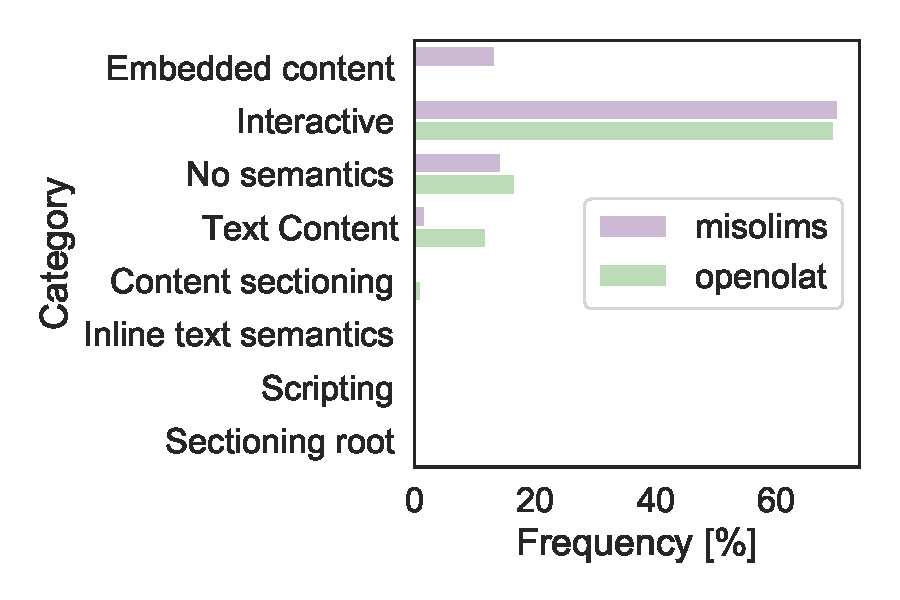
\includegraphics[width=0.45\textwidth]{figures/hpath/category-target-frequency.pdf}\label{fig:hpath-results-frequency-target}}
\subfloat[Present in DOM]{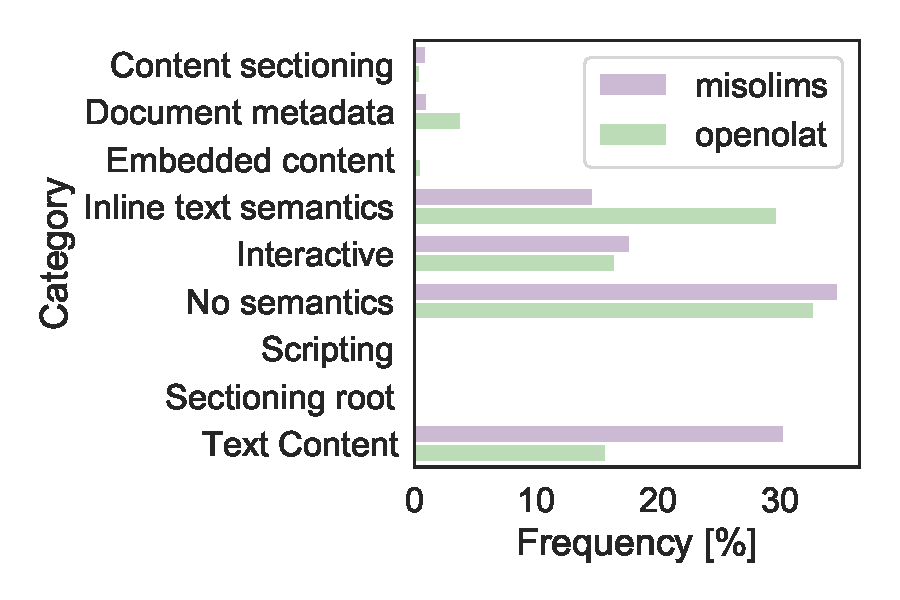
\includegraphics[width=0.45\textwidth]{figures/hpath/category-dom-frequency.pdf}\label{fig:hpath-results-frequency-dom}}
\caption{Percentages of elements (a) targeted by GUI-based tests and (b) present in the DOM for MISO LIMS and OpenOLAT across all versions aggregated by category.}  
\label{fig:hpath-results-frequency}
\end{figure}

In this research question we evaluate the prevalence of each type of element targeted by \gls{gui} tests. Indeed, HPath makes strong assumptions about the type of elements being targeted by tests. For instance, elements from the Inline Text Semantics category and elements with no semantic attached ($E_{div}$ and $E_{span}$) that are not rendered cannot be reached by our approach. Furthermore, two (\emph{label} and \emph{text}) out of the four predicates present in the current implementation specifically target elements of the Interactive category. The institution behind these assumptions is that \gls{gui} tests interact with the application in the same fashion as a user would, through visible \gls{gui} components. 

Figure~\ref{fig:hpath-results-frequency} presents the distribution of target elements grouped by their semantic categories. It contrasts the frequency of elements targeted by \gls{gui} tests (Figure~\ref{fig:hpath-results-frequency-target}) to their overall frequency in the HTML document (Figure~\ref{fig:hpath-results-frequency-dom}). The discrepancy between the two shows that not all elements are of interest to testers. Indeed, the most prevalent categories in the HTML documents are No Semantics with 34.77\% and 32.82\% for MISO LIMS and OpenOLAT respectively, Inline Text Semantics with 29.76\% for OpenOLAT and Text Content with 30.32\% for MISO LIMS. However, Figure~\ref{fig:hpath-results-frequency-target} shows a very different picture, where the overwhelming category is Interactive with 70.27\% and 69.70\% for MISO LIMS and OpenOLAT respectively, confirming our hypothesis.

However, looking at Figure~\ref{fig:hpath-results-frequency-target} we observe a non-negligible amount of elements with no semantics accounting for 14.45\% in MISO LIMS and 16.71\% in OpenOLAT. After reviewing the tests it appears that some assertions and synchronization points target portions of the \gls{dom} defined by a $e_{div}$. Therefore, while they do not hold any intrinsic semantic in the HTML standard they do act as an anchor point that can be targeted by test scripts to assess the presence of an underlying group of elements. A more detailed discussion is presented in Section~\ref{sec:hpath-results-rq2} regarding the impact on HPath.

Finally, two categories vary from one project to the other, namely, Embedded content and Text content. The presence of elements from the Embedded content in MISO LIMS (13.41\%) is explained by clickable images under an anchor element, thus behaving like Interactive Elements. As for the elements from Text Content category present in OpenOLAT (11.91\%), they are used when asserting that the \gls{sut} is in the expected state, thus, following our hypothesis.

To conclude this research question, we see that \gls{gui} tests typically target specific portions of the HTML document, namely, Interactive elements and visible components on the page (text and images). HPath, relies on relevant properties to specify these elements and offers good predicates when locating them. However, the proportion of target elements with no HTML semantic is not negligible, which could make HPath enable to locate these elements if they are not rendered on the screen. We investigate this possibility in the next research question. 

\subsection{RQ2: Element Properties Used by Locators}
\label{sec:hpath-results-rq2}

This research question investigates the relative performance in exploiting properties of target elements in the location path. HPath, absolute XPath and Robula+ formulating different hypotheses on which properties of an element can be used to locate it, we compare the three approaches.

Before being able to analyze which properties of the \gls{dom} HPath can leverage, we need to ensure that the target elements are reachable by the technique. Indeed, as shown in Section~\ref{sec:hpath-results-rq1} around 15\% of the target elements might not be rendered on the page. It appears that HPath fails to retrieve the locator in 11.58\% of the cases for MISO LIMS and in 10.48\% for OpenOLAT. These target elements not being rendered on the page, HPath is enabled to retrieve them. When observing the data, we see that assertions and synchronization points can target $e_{div}$ to verify the presence of the underlying group of elements. However, in many cases, other elements could have been selected to yield the same result had the initial test automation engineer relied on HPath. For example, in the project OpenOLAT, a test waits for a calendar widget to be rendered on a page, thus waits for the containing $e_{div}$ identified by its id (fc-view-container). The widget offering a series of named buttons (monat, tag, jhar) the test could rely on those to assess the availability of the widget. In the remaining of the discussion, only elements reachable by HPath are considered.

\begin{figure}
\centering
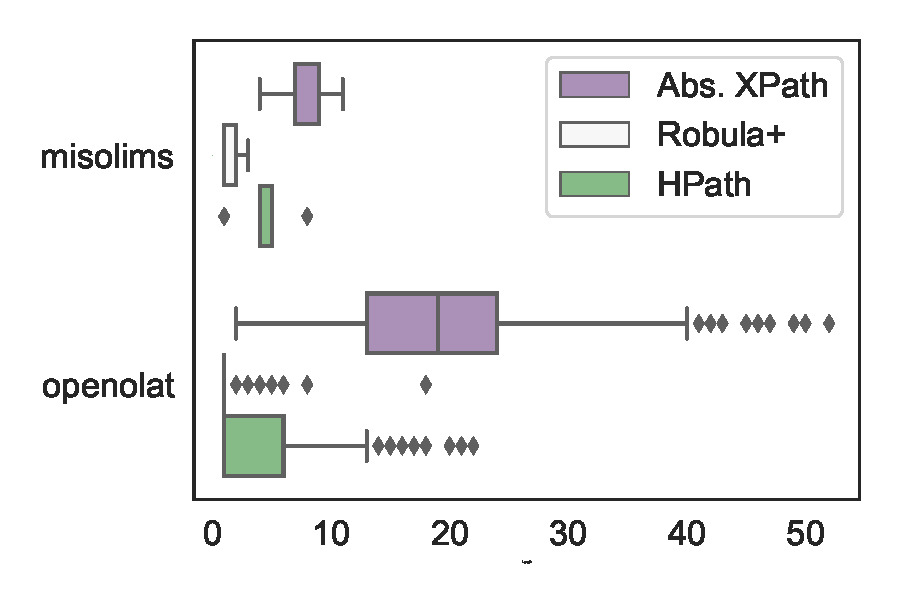
\includegraphics[width=0.6\columnwidth]{figures/hpath/canonical-selector-complexity-dist.pdf}
\caption{Length of absolute XPath, HPath and Robula+ for MISO LIMS and OpenOLAT across all versions.}  
\label{fig:hpath-results-lengths}
\end{figure}

We can now start our discussion on the properties by analyzing how much of the tree hierarchy is leaked when generating the location path. Figure~\ref{fig:hpath-results-lengths} displays the distribution of the length of the locators for the three strategies: absolute XPath, $L_{AXPath}$, Robula+, $L_{Robula+}$, and HPath, $L_{HPath}$. The figure shows a similar trend in both projects where absolute XPath yields the longest location paths with an average length of 8.6 and 18.7, Robula+ the shortest location path, with 1.6 and 1.0 and HPath lies between the two with 4.4 and 3.1, for MISO LIMS and OpenOLAT respectively. The lower performances of absolute XPath are to be expected since if no optimization can be done, both Robula+ and HPath generate a location path that is equal to the absolute XPath. Therefore $L_{HPath} \leq L_{AXPath}$ and $L_{Robula+} \leq L_{AXPath}$.

We compare the different distributions $L_{AXPath}$, $L_{Robula+}$ and $L_{HPath}$ using statistical Wilcoxon signed-rank test\footnote{Shapiro-Wilk test ($\alpha=0.001$) shows the non-normality of the distribution} ($\alpha=0.001$). The goal of this test is to assess whether or not there exists a statistical difference between the pairwise distributions. The results show that there is indeed a difference between all distributions, hence, the different strategies yield locators with different lengths. Then, we compute the pairwise effect size to determine how often lengths from one distribution are greater than in the other. The results show that in all the cases, the size effect is close to 1, \ie\ all samples from one distribution are greater than in the other, with the exception of $L_{HPath}$ and $L_{Robula+}$ for the OpenOLAT project where the size effect is 0.68. This is due to the fact that in many cases (58.52\% for HPath and 97.72\% for Robula+) both strategies manage to generate a location path of size 1, \ie\ not leaking hierarchy details of the \gls{dom}.

Asides from the predicates, to other effects contributes to the longer length of HPath when compared to Robula+. First, in its current form, if no predicate is generated, HPath generates an absolute path. However, Robula+, always discards the root node $e_{html}$ and often $e_{body}$ since they are unique in the \gls{html} document. Thus, HPath, can reduce its length the same way with no impact on its performance or changes in its assumption. Furthermore, if a \emph{tag} is unique in the document, Robula+ creates a relative path from it, since it can directly be targeted. However, except for a few elements ($e_{html}$, $e_{body}$, $e_{head}$) the \gls{html} standard does guarantee uniqueness. This can be seen as a limitation regarding robustness against change, where the addition of a second element of the same type can break the locator.

To conclude this discussion on the length of the location paths, we can see that strategies relying on different properties yield locators with different lengths. Relying on element attributes generates the shortest location path and HPath exhibits better performances for OpenOLAT than MISO LIMS, even though the tree is deeper (as shown by the length of the absolute XPath). This is a consequence of OpenOLAT using the HTML5 standard, where MISO LIMS implements HTML4, offering more opportunities for HPath to generate good predicates.

\begin{table}
\centering
\caption{Properties of the context element leveraged by HPath and Robula+ predicates. \emph{Count} is the number of locators using a property as a predicate and \emph{\%} is the percentage among all the locators collected.}
\label{tab:hpath-results-properties}
\begin{tabular}{>{\raggedright}m{0.4in}>{\raggedright}m{0.5in}>{\raggedleft}m{0.4in} >{\raggedleft}m{0.4in}>{\raggedleft}m{0.5in} >{\raggedleft}m{0.4in}}
\toprule
\textbf{\scriptsize{Strategy}} & \textbf{\scriptsize{Property}} & \multicolumn{2}{c}{\textbf{\scriptsize{MISO LIMS}}} & \multicolumn{2}{c}{\textbf{\scriptsize{OpenOLAT}}}\tabularnewline
&   & \textbf{\scriptsize{Count}} & \textbf{\scriptsize{\%}} & \textbf{\scriptsize{Count}} & \textbf{\scriptsize{\%}}\tabularnewline
\toprule
\scriptsize{\textit{HPath}} & \scriptsize{\textit{caption}} & \scriptsize{0} & \scriptsize{0.00} & \scriptsize{0} & \scriptsize{0.00}\tabularnewline
& \scriptsize{\textit{figcaption}} & \scriptsize{0} & \scriptsize{0.00} & \scriptsize{0} & \scriptsize{0.00}\tabularnewline
& \scriptsize{\textit{label}} & \scriptsize{0} & \scriptsize{0.00} & \scriptsize{31,048} & \scriptsize{16.03}\tabularnewline
& \scriptsize{\textit{legend}} & \scriptsize{0} & \scriptsize{0.00} & \scriptsize{22,354} & \scriptsize{11.54}\tabularnewline
& \scriptsize{\textit{text}} & \scriptsize{227} & \scriptsize{1.64} & \scriptsize{93,031} & \scriptsize{48.02}\tabularnewline
& \scriptsize{\textit{\textbf{total}}} & \scriptsize{\textbf{227}} & \scriptsize{\textbf{1.64}} & \scriptsize{\textbf{142,103}} & \scriptsize{\textbf{73.35}}\tabularnewline
\hline
\scriptsize{\textit{Robula+}} & \scriptsize{\textit{id attr.}} & \scriptsize{5,161} & \scriptsize{32.93} & \scriptsize{143,334} & \scriptsize{66.23}\tabularnewline
& \scriptsize{\textit{class attr.}} & \scriptsize{412} & \scriptsize{2.63} & \scriptsize{48,483} & \scriptsize{22.40}\tabularnewline
& \scriptsize{\textit{name attr.}} & \scriptsize{207} & \scriptsize{1.32} & \scriptsize{150} & \scriptsize{0.07}\tabularnewline
& \scriptsize{\textit{title attr.}} & \scriptsize{0} & \scriptsize{0.00} & \scriptsize{3,094} & \scriptsize{1.43}\tabularnewline
& \scriptsize{\textit{text}} & \scriptsize{0} & \scriptsize{0.00} & \scriptsize{17751} & \scriptsize{8.20}\tabularnewline
& \scriptsize{\textit{\textbf{total}}} & \scriptsize{\textbf{5780}} & \scriptsize{\textbf{36.88}} & \scriptsize{\textbf{212558}} & \scriptsize{\textbf{99.80}}\tabularnewline
\bottomrule
\end{tabular}
\end{table}

Therefore, we conduct a fine-grained analysis to understand which properties HPath and Robula+ are able to leverage to compute the location path. Table~\ref{tab:hpath-results-properties} shows which element properties are exploited in the predicates of both approaches. Where HPath relies on properties from the HTML5 semantics, Robula+ exploits mainly attributes of the context element to generate the predicate.

Rows \emph{total} from Table~\ref{tab:hpath-results-properties} indicates how often a strategy is able to compute a predicate. We can see that in the case of OpenOLAT, both strategies often manage to compute predicate (73.35\% for HPath and 99.80\% for Robula+) but a lot less often in the case of MISO LIMS (1.64\% for HPath and 36.88\% for Robula+). Putting the results for MISO LIMS in contrast with the ones presented in Figure~\ref{fig:hpath-results-lengths}, we see that both strategies rely on other mechanisms to reduce the length. HPath relies on the rendering tree to prune $e_{div}$ that are not rendered. On the other hand, Robula+ during each refinement step evaluates the current location path to see if it uniquely identifies the target element. Doing so, it is able to take advantages of the fact that some element types are unique in the document, leading to location path such as "\texttt{//img}" in documents containing a single $e_{img}$ and manages to create a relative path 100\% of the time. But again, relying on the uniqueness of an element type in a document can lead to locator breakages during \gls{sut} evolution.

The next point of our discussion addresses the type of predicate used by HPath. As expected, in the case of MISO LIMS, all predicates targeting \gls{html}5 semantic elements cannot be leveraged and only the label property is used. In the case of OpenOLAT, two types of predicates are never used: \emph{caption} and \emph{figcaption}. Analyzing the \gls{html} documents, it appears that none of them contain elements $e_{caption}$ or $e_{figcaption}$. The three remaining predicates \emph{label}, \emph{legend} and \emph{text} are all related to forms ($E_{legend}$) and interactive elements ($E_{label}$ and $N_{text}$ child of Interactive element) and can be successfully used by the HPath predicate.

Robula+ on the other hands relies on the attributes of the element to compute the predicate. We see that almost all the elements of OpenOLAT offer at least one attribute that can be used (91.60\%). However, in 8.20\% of the cases, Robula+ relies on the text contained in the element. Note that the text extraction of Robula+ consists in retrieving the content the child $n_{text}$ of the context element where HPath is relying on the process described in Section~\ref{sec:hpath-hpath-text-extraction}.

In conclusion, results show that HPath is able to compute a location path in 90\% of the cases and when \gls{html}5 semantics are available in the \gls{html} document, HPath is able to successfully compute predicates for over 70\% of target elements. In the cases where no \gls{html}5 semantic is available HPath is still able to reduce the length of the location path by relying on the rendering tree it computes. Furthermore, even though relying on attributes properties offer more opportunities to generate predicate, we argue that those properties are less resistant to change in the \gls{sut}. Thus, we investigate this claim in the next research question.

\subsection{RQ3: Locators Resilience to SUT Evolution}
\label{sec:locator_evolution_analysis_results}

This third research question evaluates the impact of changes in the \gls{sut} on \gls{dom}-based locators. Relying on the methodology described in Section~\ref{sec:hpath-protocol-breakage-detection}, we present in Table~\ref{tab:locator_breakage} the percentage of locators breakage following \gls{sut} evolution. 

The results show that the two projects have very different profiles. Indeed, locator breakages depending on the type of the properties evolving in the \gls{sut}, they may vary from one development cycle to the next. However, note that the two projects are quite mature with over 15,000 commits in almost 10 years for OpenOLAT and over 4,200 commits in 9 years for MISO LIMS. This explains why no deep structural changes are observed over the periods we analyze as the low breakage count for absolute XPath suggests. Our goal being to spot iso-functional locator breakages, this stability ensures that when a breakage is observed, it is not due to a deep functional evolution of the page.

From Table~\ref{tab:locator_breakage}, for MISO LIMS, Robula+ has the lowest number of breakages (10) and closely followed by HPath (26). Figure~\ref{fig:changes_intersect_misolims} shows the intersection of elements for which the locators break. It shows that absolute XPath is a superset of Robula+ and HPath suggesting that they only break following a change in the \gls{dom} hierarchy. Furthermore, there is no overlap between Robula+ and HPath, meaning that relying on different properties make the locators resilient to different types of \gls{sut} evolution (supporting the results from \textcite{Leotta2015}).

On the other hand, the OpenOLAT project offers a very different picture. When constructing the HTML document to serve to the client, the backend of OpenOLAT automatically generates id, based on the version of the project, in order to ease communication with the database management system. HPath offers in this case the best resilience to change breaking only 0.49\% of the time. Contrarily, Robula+, relying on element attributes, offers very poor performance breaking in 64.99\% of the cases. Figure~\ref{fig:changes_intersect_misolims} shows that there exists an overlap between the different strategies but that in general they all react differently to changes.

\begin{table}
\centering
\caption{Locator breakages due to SUT evolution. \emph{Count} is the number of locators that broke because of a change and \emph{\%} is the percentage among all the pairs collected.}
\label{tab:locator_breakage}
\begin{tabular}{>{\raggedright}m{0.6in}>{\raggedleft}m{0.4in} >{\raggedleft}m{0.2in}>{\raggedleft}m{0.4in} >{\raggedleft}m{0.2in}}
\toprule
\textbf{\scriptsize{Strategy}} & \multicolumn{2}{c}{\textbf{\scriptsize{MISO LIMS}}} & \multicolumn{2}{c}{\textbf{\scriptsize{OpenOLAT}}}\tabularnewline
    & \textbf{\scriptsize{Count}} & \textbf{\scriptsize{\%}} & \textbf{\scriptsize{Count}} & \textbf{\scriptsize{\%}}\tabularnewline
\toprule
\scriptsize{\textit{Abs. XPath}} & \scriptsize{56} & \scriptsize{2.02} & \scriptsize{174} & \scriptsize{0.63}\tabularnewline
\scriptsize{\textit{Robula+}} & \scriptsize{10} & \scriptsize{0.36} & \scriptsize{17976} & \scriptsize{64.99}\tabularnewline
\scriptsize{\textit{HPath}} & \scriptsize{26} & \scriptsize{0.94} & \scriptsize{135} & \scriptsize{0.49}\tabularnewline
\bottomrule
\end{tabular}
\end{table}

\begin{figure}
\centering
\subfloat[MISO LIMS]{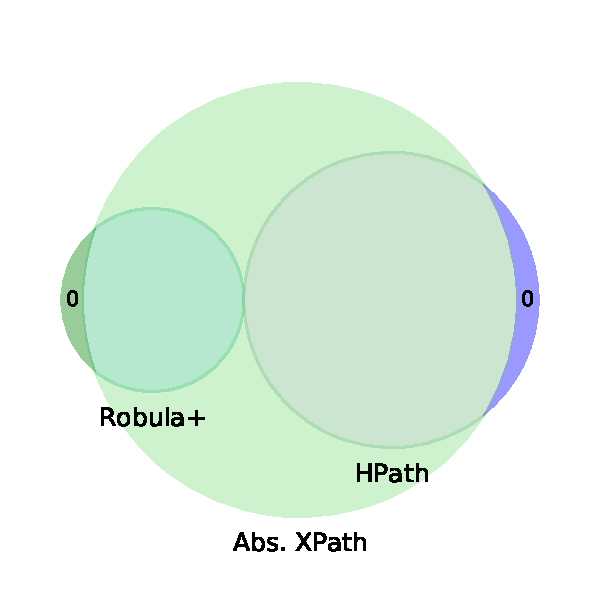
\includegraphics[width=0.45\columnwidth]{figures/hpath/changes-intersect-misolims.pdf}\label{fig:changes_intersect_misolims}}
\subfloat[OpenOLAT]{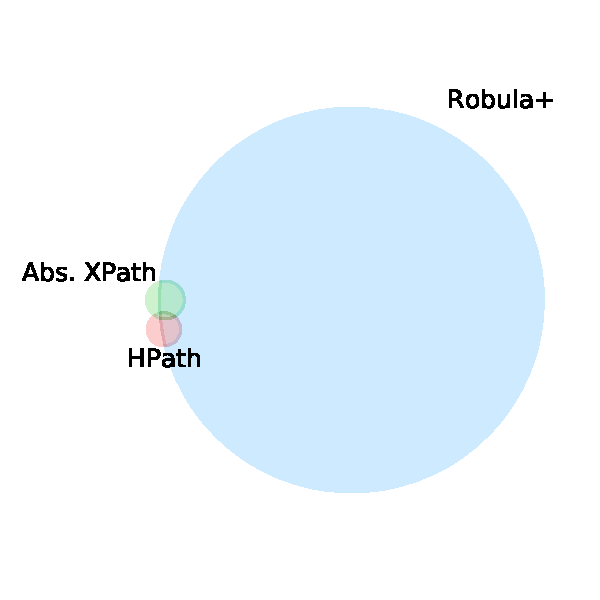
\includegraphics[width=0.45\columnwidth]{figures/hpath/changes-intersect-openolat.pdf}\label{fig:changes_intersect_openolat}}
\caption{Overlap of locators having breakage for Absolute XPath (green), Robula+ (blue) and HPath (red).}  
\label{fig:changes_intersect}
\end{figure}

To better understand which properties of the elements causes the locators to break, Table~\ref{tab:breakage_cause} shows the origin of the failure of the locator. To compute the origin, we compared the breaking location path from  $version_A$ to the passing one computed from $version_B$. The results of the fine-grain difference algorithm between the pair of locators point out the cause of the breakage. 

In the case of MISO LIMS, most of the failures happened in the position predicate, this related to the hierarchy structure of the \gls{dom}. Again, in the case of OpenOLAT, the profile is more diverse. Robula+ is not affected by changes in the element types (NameTest) in comparison to the other approaches, but is sensitive to attributes changes, leading to poor resilience to the evolution of the \gls{sut} where breakage due to the id contributed to 97.61\% of the breakage. Finally, when HPath is able to compute a predicate, it is resilient and never breaks in our dataset (Row \emph{Any Predicate} from Table~\ref{tab:breakage_cause}).  

\begin{table}
\centering
\caption{Properties causing locator breakages. \emph{Count} is the number of locators breaking because of a property and \emph{\%} is the percentage among all the breaking locators for that strategy.}
\label{tab:breakage_cause}
\begin{tabular}{>{\raggedright}m{0.6in}>{\raggedright}m{1.2in}>{\raggedleft}m{0.25in} >{\raggedleft}m{0.4in}>{\raggedleft}m{0.4in} >{\raggedleft}m{0.4in}}
\toprule
\textbf{\scriptsize{Strategy}} & \textbf{\scriptsize{Cause}} & \multicolumn{2}{c}{\textbf{\scriptsize{MISO LIMS}}} & \multicolumn{2}{c}{\textbf{\scriptsize{OpenOLAT}}}\tabularnewline
 &   & \textbf{\scriptsize{Count}} & \textbf{\scriptsize{\%}} & \textbf{\scriptsize{Count}} & \textbf{\scriptsize{\%}}\tabularnewline
\toprule
\scriptsize{\textit{Abs. XPath}} & \scriptsize{\textit{NameTest}} & \scriptsize{0} & \scriptsize{0.00} & \scriptsize{60} & \scriptsize{34.48}\tabularnewline
 & \scriptsize{\textit{Predicate position}} & \scriptsize{56} & \scriptsize{100.00} & \scriptsize{114} & \scriptsize{65.52}\tabularnewline
 \hline
\scriptsize{\textit{Robula+}} & \scriptsize{\textit{NameTest}} & \scriptsize{0} & \scriptsize{0} & \scriptsize{11} & \scriptsize{0.06}\tabularnewline
 & \scriptsize{\textit{Predicate position}} & \scriptsize{10} & \scriptsize{100.00} & \scriptsize{2} & \scriptsize{0.01}\tabularnewline
 & \scriptsize{\textit{Predicate id attr.}} & \scriptsize{0} & \scriptsize{0.00} & \scriptsize{17,578} & \scriptsize{97.79}\tabularnewline
 & \scriptsize{\textit{Predicate class attr.}} & \scriptsize{0} & \scriptsize{0.00} & \scriptsize{11} & \scriptsize{0.06}\tabularnewline
 & \scriptsize{\textit{Predicate title attr.}} & \scriptsize{0} & \scriptsize{0.00} & \scriptsize{77} & \scriptsize{0.43}\tabularnewline
 & \scriptsize{\textit{Predicate text content}} & \scriptsize{0} & \scriptsize{0.00} & \scriptsize{281} & \scriptsize{1.56}\tabularnewline
 \hline
\scriptsize{\textit{HPath}} & \scriptsize{\textit{NameTest}} & \scriptsize{0} & \scriptsize{0.00} & \scriptsize{119} & \scriptsize{88.14}\tabularnewline
 & \scriptsize{\textit{Predicate position}} & \scriptsize{26} & \scriptsize{100.00} & \scriptsize{16} & \scriptsize{11.85}\tabularnewline
 & \scriptsize{\textit{Any Predicate}} & \scriptsize{0} & \scriptsize{0.00} & \scriptsize{0} & \scriptsize{0.00}\tabularnewline
\bottomrule
\end{tabular}
\end{table}

In conclusion, when HPath can generate predicates they lead to robust and flexible locators. However, it can be hard for the approach to extract the necessary properties as shown in section~\ref{sec:locator_evolution_analysis_results}. Therefore, while the results are promising, more research needs to be conducted to better exploit the rendering properties present in the HTML5 semantics. Furthermore, better reliance on the standard by developers would improve the performances of tool relying on the semantic of the language.
\section{Threats to Validity}

The internal threat to validity concerns the way evolution are computed. During our analysis of the \gls{html} document pairs, we realized that some pair only vary by a date or a timestamp unrelated to any of the targeted elements. While decrease the overall percentage of breakage, because this effect is similar for all techniques, it does not have any effect on neither the ranking of the methods nor the number of breakages observed.

Furthermore, when we observe a breakage, we do not have guarantie of the iso-functionality of the \gls{gui} element being targeted. Indeed, if the element is deeply modify or it might be expected for the locator to break. We limit the impact of this effect by using the Absolute XPath as a baseline and by ensuring that in the two versions the same test was executed against the \gls{sut}.

Finally, conducting our case study on two projects, the conclusions we draw may not hold true for other projects. This constitutes a major threat to the external validity for the generalization of our results outside the context of this study. However, the two projects have very different profiles, thus making the study covering boundary cases among the full range of possible projects. To further alleviate this limitation, we encourage other teams to replicate and extend our results.


	\chapter{Ikora Framework}
\label{chap:ikora-framework}
	\section{Conclusions}

We presented HPath, a novel DOM-based locator strategy to generate location paths more flexible for web testing. We have compared its potential to extract properties from the HTML document and its fragility under SUT evolution against state-of-the-art algorithm Robula+. Our results show that when HTML5 semantics are present, HPath can exploit rendered properties of web elements to generate expressive locators in 73.35\% reducing locator breakages from 64.99\% when relying on attribute properties to 0.49\% with rendered properties. However, in its current form, it is not always able to extract rendered properties to create good location paths and leaks the hierarchical structure of the DOM for 41.48\% of the elements.

While HPath offers clear advantages in its expressiveness (only relying on rendered properties) and flexibility (when compared to Robula+), it suffers from some limitations. Indeed, relying on very specific predicates, the approach is not always able to generate short and expressive location paths, which might expose more of the internal hierarchy of the \gls{html} document. This effect is exacerbated when the targeted page is not relying on the current \gls{html}5 standards. However, despite this limitation, our results show that relying on the structure of the rendered \gls{dom} still remains better than exploiting the internal attributes of the elements from the \gls{html} document.
	
	\backmatter
\end{document}